% !TeX encoding = UTF-8
\documentclass[bind,a4paper]{mythesis}

\usepackage{thesis}
%\usepackage[full,round]{harvard}%
\usepackage{natbib}%\bibpunct{(}{)}{;}{a}{,}{,}
\usepackage{pgfplots}
\usepackage{graphicx}
\usepackage{latexsym}
\usepackage{verbatim}
%\usepackage[latin1]{inputenc}
\usepackage[brazilian]{babel}
\usepackage[utf8]{inputenc}
\usepackage{amssymb}
\usepackage{amsmath}
\usepackage{amstext}
\usepackage{amscd}
\usepackage{amsthm}
\usepackage{fancyhdr,fancybox}
\usepackage{psfrag}
\usepackage{rotating}
\usepackage{url}
%\usepackage[colorlinks]{hyperref}
%\usepackage{listings}
\usepackage{epstopdf}
\usepackage{makeidx}
\usepackage{authorindex}
\usepackage{multirow}
\usepackage{picture}
\usepackage[algochapter,algoruled,linesnumbered,vlined,portugues]{algorithm2e}
\usepackage{algorithmic2e}
%\usepackage{rotating}
\usepackage{tocbibind}
\usepackage{array}
\usepackage{lscape}
%\usepackage{ragged2e}

%\usepackage[ruled,vlined,portuguese]{algorithm2e}
\usepackage{rotating}
\usepackage{longtable}
\usepackage{listings}
\usepackage{graphicx}
\usepackage{url}
\usepackage{cancel}
\usepackage{scalefnt}
\usepackage{todonotes}
\usepackage{wrapfig}

\usepackage{float}
\restylefloat{figure}
%\usepackage[T1]{fontenc}
%\input{tex/defs.tex}
\makeindex

\newcommand{\listofalgorithmes}{\tocfile{\listalgorithmcfname}{loa}}

\newcommand{\hardware }{\textit{hardware}}
\newcommand{\Hardware }{\textit{Hardware}}
\newcommand{\software }{\textit{software}}
\newcommand{\Software }{\textit{Software}}
\newcommand{\hardwares}{\textit{hardwares}}
\newcommand{\Hardwares}{\textit{Hardwares}}
\newcommand{\softwares}{\textit{softwares}}
\newcommand{\Softwares}{\textit{Softwares}}

\newcommand{\hs}{\textit{hardware}\ e\ \textit{software}}
\newcommand{\HS}{\textit{Hardware}\ e\ \textit{Software}}

\newcommand{\wearable} {\textit{wearable}}
\newcommand{\Wearable} {\textit{Wearable}}
\newcommand{\wearables}{\textit{wearables}}
\newcommand{\Wearables}{\textit{Wearables}}


\newcommand{\design}   {\textit{design}}
\newcommand{\designer} {\textit{designer}}
\newcommand{\Design}   {\textit{Design}}
\newcommand{\Designer} {\textit{Designer}}
\newcommand{\designs}  {\textit{designs}}
\newcommand{\designers}{\textit{designsers}}
\newcommand{\Designs}  {\textit{Designs}}
\newcommand{\Designers}{\textit{Designers}}
\newcommand{\assembly} {\textit{assembly}}
\newcommand{\profile}  {\textit{profile}}
\newcommand{\Profile}  {\textit{Profile}}
\newcommand{\speedup}  {\textit{speedup}}
\newcommand{\Speedup}  {\textit{Speedup}}
\newcommand{\core}     {\textit{core}}
\newcommand{\cores}    {\textit{cores}}
\newcommand{\codesign} {\textit{codesign}}
\newcommand{\mobile}   {\textit{mobile}}
\newcommand{\benchmark}   {\textit{benchmark}}
\newcommand{\benchmarks}   {\textit{benchmarks}}
\newcommand{\Benchmark}   {\textit{Benchmark}}
\newcommand{\Benchmarks}   {\textit{Benchmarks}}

\newcommand{\A}{$\mathcal{A}$}
\newcommand{\B}{$\mathcal{B}$}
\newcommand{\C}{$\mathcal{C}$}

\newenvironment{VarDescription}[1]%
  {\begin{list}{}{\renewcommand{\makelabel}[1]{\hspace{0cm}\hfil\textbf{##1}  :}%
    \settowidth{\labelwidth}{\hspace{0cm}\textbf{#1} :}%
    \setlength{\leftmargin}{\labelwidth}\addtolength{\leftmargin}{\labelsep}}}%
  {\end{list}}

\newcounter{matriz}
\newenvironment{matriz}{\refstepcounter{matriz}\equation}{\tag{M\thematriz}\endequation}


%\input{macros}

%% PDF metadata
\makeatletter
\@ifpackageloaded{hyperref}{%
  \hypersetup{%
  colorlinks=false,
  pdftitle = {Uma Abordagem do Problema de Particionamento \Hardware\ e \Software\ para \Design\ de Sistemas Computacionais \Wearables},
  pdfsubject = {Rodolfo Labiapari Mansur Guimarães's MsC thesis},
  pdfkeywords = {Wearable, FPGA, Hardware Software Partitioning},
  pdfauthor = {\textcopyright\ Rodolfo Labiapari Mansur Guimarães}}
}{}
\makeatother

%Hyphenations
\hyphenation{XHSTT}
%\hyphenation{res-tri-ções}
\hyphenation{co-nhe-ci-do}
\hyphenation{co-nhe-ci-da}
\hyphenation{re-a-li-za}
\hyphenation{vi-zi-nho}
\hyphenation{clim-bing}
\hyphenation{ran-king}
\hyphenation{me-lhor}
\hyphenation{ou-tras}
\hyphenation{ge-ra-das}
\hyphenation{ex-pe-ri-men-tos}
\hyphenation{pro-ble-ma}
%\hyphenation{su-ges-tões}
\hyphenation{pos-te-rior-men-te}


%% Define the thesis title and author
\begin{document}
\let\cleardoublepage\clearpage
\title{Uma Abordagem do Problema de Particionamento \Hardware\ e \Software\ para \Design\ de Sistemas Computacionais \Wearables\ ANTIGASSSSÇÇÇÇÇÇOOOOOOOOOOOOO}
\author{Rodolfo Labiapari Mansur Guimarães}%% Start the document

%% Define the un-numbered front matter (cover pages, rubrik and table of contents)
\begin{frontmatter}
	\selectlanguage{brazilian}
	%!TEX root = ../main_text.tex
\let\cleardoublepage\clearpage
\titlepage[Universidade Federal de Ouro Preto]{

\vspace{-21cm}
\textbf{UNIVERSIDADE FEDERAL DE OURO PRETO}

\vspace{13cm}

Orientador: Dr. Ricardo Augusto Rabelo Oliveira \\ \vskip8pt

\vspace{3cm}

\hspace{7.5cm}
\parbox{0.5\textwidth}{
Dissertação submetida ao Instituto
de Ciências Exatas e Biológicas da Universidade
Federal de Ouro Preto para qualificação ao
título de Mestre em Ciência da Computação
}

\vspace{2.8cm}

\begin{center}
Ouro Preto, Setembro de 2017
\end{center}
}

\let\cleardoublepage\clearpage

\titlepage[Universidade Federal de Ouro Preto]{
\vspace{-21cm}
\textbf{}
\vspace{13cm}

Orientador: Dr. Ricardo Augusto Rabelo Oliveira \\ \vskip8pt

\vspace{3cm}

\begin{figure}[h!]
  \begin{center}
    
\includegraphics[width=1.0\textwidth]{img/logo.png}
    \label{fig:goal}
  \end{center}
\end{figure}

}

%\begin{figure}[h]
 % \begin{center}
  %  \includegraphics[width=1.0\textwidth]{img/ataDefesa.pdf}
   % \label{fig:ataDefesa}
  %\end{center}
%\end{figure}

\begin{comment}

\dedication{\vspace{4cm}
\begin{flushright}
Dedico este trabalho a você que sempre me fez acreditar na realização dos meus sonhos e trabalhou muito para que eu pudesse realizá-los, \emph{Mãe}. A minha \emph{família} e \emph{amigos} que sempre me apoiaram nas horas difíceis. Ao meu \emph{pai}, que mesmo distante influenciou para que pudesse chegar até aqui.

\end{flushright}

}
\end{comment}

%% Abstract in portuguese
\begin{abstract}[\smaller \titulo\\ \vspace*{1cm} \smaller Resumo]
  %\thispagestyle{empty}


Este trabalho constitui-se de uma abordagem do problema de particionamento \hs\ para dispositivos vestíveis com foco em aumento de performance, visando o gasto de recursos em seu \textit{trade-off}.
A tecnologia digital de fatores como microeletrônica, sensores e comunicação móvel são constantemente melhoradas à medida que a informação torna-se cada vez mais sem-fio, tornando-a um grande estímulo para o desenvolvimento de dispositivos inteligentes e conectados como sistemas embarcados IoT ou vestíveis (do inglês \wearables). 
Isso é visto no rápido desenvolvimento de dispositivos para comércio, entretanto, ainda com a dificuldade de satisfazer os requerimentos das várias aplicações modernas. 
Tais dispositivos utilizam de um leque enorme de sensores e necessitam de um serviço autônomo, o que implica numa grande demanda de performance somado com o baixo consumo de energia sem deixar design, segurança e confiabilidade a desejar. 
Para obter um produto de alta qualidade, atendendo aos requisitos solicitados, esta pesquisa consiste na análise de projetos para sistemas \wearables\ utilizando plataformas FPGA como meio na realização de particionamentos \hs\ obtendo um bom \speedup\ e eficiência em comparação a outros sistemas como \textit{in-software}. 
%Com mais pesquisas voltadas para saúde e conforto humano, os dispositivos \wearables\ estão possuindo cada vez mais habilidades para detectar e identificar pessoas ou seus comportamentos e assim tornar um complemento/auxílio para as atividades cotidianas.

%To adequately address these demands, sophisticated embedded computing and embedded design technologies are needed. After an introduction to modern mobile systems, this paper discusses the huge heterogeneous area of these systems, and considers serious issues and challenges in their design. Subsequently, it discusses the embedded computing and design technologies needed to adequately address the issues and overcome the challenges in order to satisfy the stringent requirements of the modern mobile systems.
Palavras-chave: Particionamento \hs, Sistema \Wearable, Sistemas Embarcados.
\end{abstract}
\let\cleardoublepage\clearpage


%% Abstract
\begin{abstract}[\smaller An Approach of Hardware and Software Partitioning Problem for the Design of Wearable Computing Systems\\ \vspace*{1cm} \smaller Abstract]

  %\thispagestyle{empty}
  
This work consists of an approach of the hardware and software partitioning problem for wearable devices focused on performance enhancement, aiming at the expense of resources in their trade-off.
The digital technology of factors such as microelectronics, sensors and mobile communication are constantly improved as information becomes increasingly wireless, making it a great stimulus for the development of intelligent and connected devices like embedded IoT or wearable systems.
This is seen in the rapid development of devices for commerce, however, still with the difficulty of satisfying the requirements of the various modern applications.
Such devices use a wide range of sensors and require autonomous service, which implies a great demand for performance coupled with low power consumption without leaving design, security and reliability to be desired.
In order to obtain a high-quality product, meeting the requested requirements, this research consists of the analysis of designs for wearables systems using FPGA platforms as a means of realizing hardware and software partitions obtaining good speedup and efficiency compared to other systems such as in-software.

Keywords: Hardware and Software Partitioning, Wearable System, Embedded System.
\end{abstract}

\begin{comment}

\let\cleardoublepage\clearpage
%% Declaration
\begin{declaration}
Esta dissertação é resultado de meu próprio trabalho, exceto onde referência explícita é feita ao trabalho de outros, e não foi submetida para outra qualificação nesta nem em outra universidade.
\vspace*{1cm}
\begin{flushright}
Danilo Santos Souza
\end{flushright}
\end{declaration}

%% Acknowledgements
\let\cleardoublepage\clearpage
\begin{acknowledgements}

Primeiramente agradeço à \emph{Deus} por me amparar nos momentos difíceis e me dar força para superar as dificuldades.

Aos meus pais, \emph{Gilsa e Denildo}, e a meu irmão \emph{Diego}, pelo incentivo, apoio e afeto.

A minha avó \emph{Carmelita}, pelo exemplo de dedicação e por ser uma mãe pra mim.

Ao meu Tio \emph{Denilson}, por sempre acreditar em mim quando alguns não acreditavam, e por ser um exemplo de pai e homem.

À toda minha \emph{família}, pelo carinho e força.

Agradeço ao meu orientador \emph{Gustavo Peixoto Silva} pela oportunidade concedida, pela impecável orientação e pelo apoio no desenvolvimento do trabalho. Agradeço ainda ao meu Coorientador \emph{Haroldo Gambini Santos} pelas valiosas contribuições para o presente trabalho.

Aos meus amigos \emph{Bruna, Priscilla, Gabriela, Thayane, Lorran, Aristides, Alisson, Pereira, Lucas, Marco, Emilia, Danielle e Flavio} pela ajuda, pelas longas horas de estudo, amizade, carinho e força, fundamentais para que eu conseguisse chegar até aqui.

À República \emph{Navio Pirata}, Moradores e Ex-alunos, por me acolherem, pelo companheirismo e amizade, tornando esta minha segunda casa.

Ao \emph{CNPq}, à \emph{FAPEMIG}, à \emph{CAPES} e à \emph{UFOP} pelo apoio recebido no desenvolvimento deste trabalho.

Ao \emph{PPGCC - UFOP}, professores e técnicos, em especial aos professores Fabrício, Gustavo e Haroldo, e a Mariana pela ajuda sempre que fez-se necessário.

Enfim, agradeço a \emph{todos} que, de alguma forma, acreditaram e torceram por mim, participaram de minha vida e ajudaram na realização deste trabalho.

\end{acknowledgements}

\end{comment}


%% Preface
%\begin{preface}
%
%\end{preface}

% ToC
\tableofcontents
\listoffigures
\let\cleardoublepage\clearpage
%\listoftables
%%\listofalgorithms
%\listofalgorithmes

\begin{comment}

%% Strictly optional!
\frontquote%
{Talvez não tenha conseguido fazer o melhor, mas lutei para que o melhor fosse feito. Não sou o que deveria ser, mas Graças a Deus, não sou o que era antes.}%
{Marthin Luther King}

\end{comment}

\end{frontmatter}

%% Start the content body of the thesis
\begin{mainmatter}
  \selectlanguage{brazilian}
  	%!TEX root = ../main_text.tex

\chapter*{Nomenclaturas}
\addcontentsline{toc}{chapter}{Nomenclatura}
\markboth{Nomenclaturas}{Nomenclaturas}

%% Nomenclature
\begin{tabular*}{20cm}{lp{12cm}}
ASIC  & \textit{Application-Specific Integrated Circuit} \\
CI    & \textit{Circuito Integrado} \\
CUDA  & \textit{Compute Unified Device Architecture} \\
CPU   & \textit{Central Processing Unit} \\
CSoC  & \textit{Configurable System on a Chip} \\
DRES  & \textit{Dynamically Reconfigurable Embedded Systems} \\
FPGA  & \textit{Field-Programmable Gate Array} \\
FPLD  & \textit{Field-Programmable Logic Device} \\
GA    & \textit{Genetic Algorithm} \\
GC    & \textit{Grafo de Chamada} \\
GFC   & \textit{Grafo de Fluxo de Controle} \\
GPU   & \textit{Graphical Processing Unit} \\
HDL   & \textit{Hardware Description Language} \\
HLS   & \textit{High-Level Synthesis} \\ 
IoT   & \textit{Internet of Things} \\
LED   & \textit{Light-Emitting Diode} \\
LUT   & \textit{Look-Up Table} \\
NRE   & \textit{Nonrecurring Engineering} \\
PLD   & \textit{Programmable-Logic Device} \\
RAM   & \textit{Random-Access Memory} \\
\end{tabular*}

\begin{tabular*}{20cm}{lp{12cm}}
   SRAM  & \textit{Static Random-Access Memory} \\
   VGA   & \textit{Video Graphics Array} \\
   VHDL  & \textit{VHSIC Hardware Description Language} \\
   VHSIC & \textit{Very High Speed Integrated Circuits} \\
\end{tabular*}

%se tiver mais de uma página usar outra tabela
%\begin{tabular*}{20cm}{lp{12cm}}
%$\emph{fem}$ & Força eletromotriz\\
%\end{tabular*}

	\let\cleardoublepage\clearpage
	% !TEX root = ../main_text.tex
% !TeX encoding = UTF-8
\chapter{Introdução} \label{chap:introducao}

   %\todo[inline]{contextualização lógica}
	%intro geralzona
	O recente progresso na obtenção e manipulação de informações, em conjunto com a ascensão da tecnologia da microeletrônica, comunicação e sensores, proporcionou um enorme estímulo no desenvolvimento de sistemas computacionais inteligentes de comunicação e \wearables, todos sendo dispositivos embarcados \citep{Jozwiak2017}.
	%
	O projeto de sistemas computacionais está mais complexo que nunca. A demanda por curto tempo para disponibilidade ao mercado, somado ao fato dos produtos exigirem propriedades de corretude, rapidez, confiabilidade e preço acessível, representam um desafio para projetistas de sistemas embarcados em geral.
	Sistemas computacionais embarcados (também nomeados pela literatura como sistemas embarcados ou sistemas embutidos) possuem muitos componentes implementados tanto em \hs\ e esta decisão de escolha de local de implementação será o tema principal abordado neste documento com foco em dispositivos \wearable.

	% embedded 
   %\todo[inline]{A parte de wearable vc tem q explorar mais no capitulo 1 tb, como construcao da motivacao. Uma introducao tem q ser a sequinte sequencia}
	Os sistemas computacionais embutidos são produtos que utilizam processadores ou controladores e podem estar desde fornos de microondas, até sistemas de controle de aeronaves.
   São computadores situados em dispositivos e que sua presença não é imediatamente óbvia.
	Requerem técnicas na qual difere das utilizadas para \design\ de computadores de propósito geral ou aplicações de \software\ dessas máquinas \citep{Wolf1994}.  
	Em 2015, foi previsto um total de 6,5 bilhões de dispositivos ativamente conectados para o ano de 2016, segundo notícias da empresa de pesquisa e consultoria Gartner \citep{RobvanderMeulen2015}.
	
	% wearable
	No âmbito de sistemas embutidos, existe um subconjunto na qual possui o propósito de integrar-se ao sistema corporal expandindo suas capacidades. 
	Esses dispositivos `vestíveis', chamados de sistemas \wearables, envolvem grande volume de dados de múltiplos sensores ou outros sistemas e são requeridos para prover serviço autônomo, contínuo, em um longo período de tempo.
   Diferentemente de \textit{smartphones} e \textit{tablets}, os \wearables\ são tecnologias eletrônicas ou computadores que são incorporados ao vestuário dos usuários criando uma integração cada vez mais intensa entre tecnologia e ser humano. 
   Sua tendência é superar os dispositivos manuais como computadores e telefones pois são dispositivos mais sofisticados pela existência de recursos sensoreais e escaneamento.
   %
   Cerca de 20\% da população possui pelo menos um dispositivo sendo que 10\% utiliza-o todos os dias \citep{lee2016information}.
   São dispositivos que permitem benefícios como um estilo de vida inspirado em dados \textit{fitness} até realidade aumentada preenchida por objetos virtuais.
	Tais dispositivos demandam de uma alta performance e/ou baixo consumo de energia, sem apresentar \textit{trade-off} de confiabilidade e segurança entre outros. % \citep{Jozwiak2017}.
	%
	Segundo o trabalho de \citet{Jozwiak2017}, com computação de alta performance e estudos em gasto energético eficiente, foi possível a facilitação do rápido progresso da computação móvel e autônoma.
	%Tudo isso deve-se à possibilidade de comunicar-se com a rede global de comunicação, combinada com o progresso de sensores e atuadores, criando novas oportunidades importantes de projeto.
	%%Exemplos disso são indústrias inteligentes, cidades e casas, bem como setores de IoT, sistemas móveis como automóveis inteligentes, computação móvel como \textit{smartphones}, comunicação e, não menos importante, os sistemas computacionais \wearable.
	Sistemas computacionais \wearables\ podem ser definidos como `embutidos que foram inseridos em ambiente \mobile\ de seus usuários, não exercendo a mesma atividade' e seu propósito é criar dispositivos com acesso constante, conveniente, portátil e principalmente \textit{hands-free}, aplicando não só na área de saúde e esportiva, mas também em entretenimento e assim por diante.

   %\todo[inline]{1- Apresnetar o problema:}
   \section{Problema}
	% intro particionamento
	A redução do ciclo de comercialização de um produto e o aumento de sua eficiência de desenvolvimento de projeto tem se tornado uma preocupação na área de \design\ de sistemas embarcados, incluindo também os \wearables.
	E por este motivo, a técnica de particionamento \hs\ tem sido uma das principais tecnologias para o desenvolvimento de sistemas embarcados em geral, desde que, este afeta a performance do sistema como um todo. 
   Para \citet{Hassine2017}, uma das soluções mais elegantes na computação que provê otimizações sistêmicas sobre essas circunstâncias é por meio do particionamento \hs.
	Segundo \citet{Wolf1994}, sistemas embutidos gerais são considerados únicos pelo fato da necessidade de um \codesign\ de \hs. 
   As pesquisas em \codesign\ de \hs\ têm como objetivo o \design\ de sistemas heterogêneos, visando performance, custo e metas de confiabilidade \citet{Edwards1994}.
	
   \begin{comment}
   
   Um exemplo simbólico de \codesign\ para o particionamento pode ser ilustrado na Figura \ref{fig:rt-edwards_partitioning} no qual um módulo em \software\ é substituído por um componente em \hardware\ executando a mesma tarefa mas com maior performance.
   
   \begin{figure}[h] \centering
   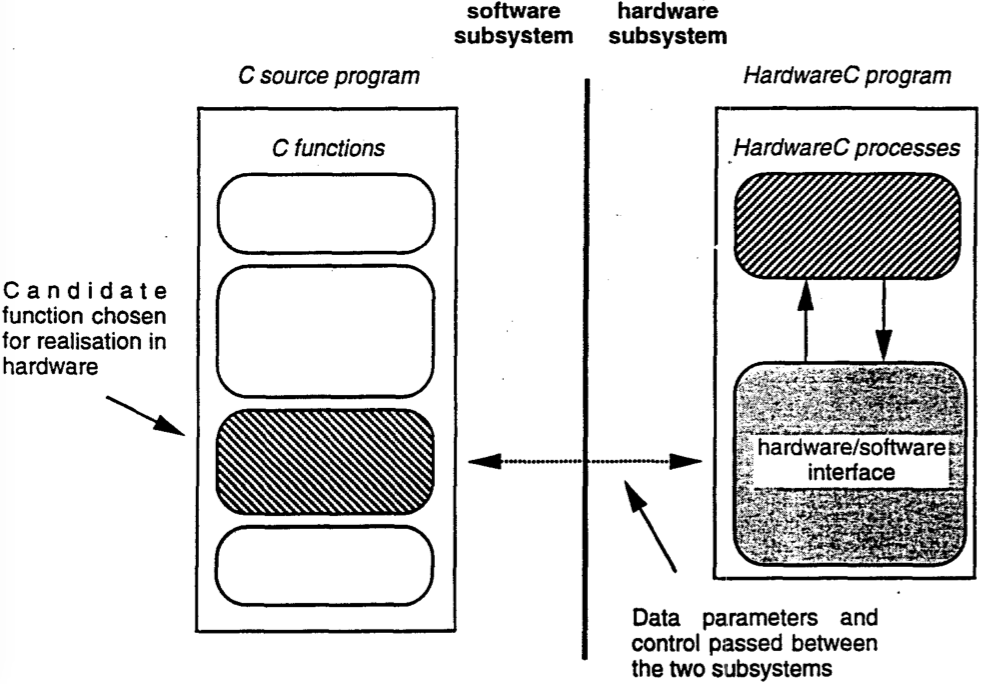
\includegraphics[width=0.7\textwidth]{img/rt-edwards_partitioning.png}
   \caption{Ilustração de um particionamento no \codesign\ de um sistema embarcado. Fonte: \citet{Edwards1994}.}
   \label{fig:rt-edwards_partitioning}
   \end{figure}
\end{comment}

	\citet{Hidalgo1997} dizem que o objetivo principal é o balanceamento de todas as tarefas de forma a otimizar alguns objetivos de sistema sobre determinadas restrições.
	Agrupar específicos conjuntos de instruções de uma aplicação e então mapear esses grupos tanto em \hs.
	%Os grupos designados ao \software\ são executados sequencialmente pelo respectivo processador do sistema enquanto os mapeados em \hardware\ são implementados por uma combinação customizada ou por circuitos sequenciais \citep{Sass2010}.

	% particionamento
	%Quando necessita de performance ao realizar o \codesign\ (termo referente ao inglês \textit{Participatory Design}) de \hs\ para sistemas embutidos, o problema de qual função do sistema deverá ser implementada em \hardware\ ou em \software\ emerge e esse problema é conhecido por particionamento \hs\ (\textit{hardware/software partitioning}).
	%Um significante esforço foi posto nesta área nos últimos dez anos, segundo \citet{Trindade2016}.
   
   Um desafio de \design\ é combinar a flexibilidade de demanda pelos vários ambientes e aplicações, e a alta performance exigida em tarefas com o baixo consumo de energia requerido para maximizar o tempo de uso da bateria.

   %\todo[inline]{3- Motivacao pra resolver este problema:}

	%Com o desenvolvimento de sistemas embutidos cada vez mais complexos, o particionamento \hs\ tornou-se um problema de otimização em \codesign\ de sistemas \citep{Yan2017}. 
   A motivação é que, tal problema que envolve \design\ colaborativo e multidisciplinar, é um passo-chave no \design\ de produtos modernos \citep{Trappey2016}. 
   Implementações que baseiam-se somente em módulos de \software\ possuem mais flexibilidade e menos custosos, entretanto, seu custo eleva-se em termos de tempo de execução. Uma implementação de \hardware\ customizada de um conjunto de computações proverá uma eficiência energética e \speedup\ maior relativa à implementações em \software\ \citep{Zhang2008, Hassine2017, Wolf1994, Canis2011, Stone2010}.

   % combinação de fpga com cpu
   A tendência hoje para \design\ é na combinação das funções do processador com os recursos dos arranjo de portas programáveis em campo (FPGAs, do inglês \textit{Field-Programmable Gates Array}) formando um sistema computacional híbrido. %, exemplo exibido na Figura \ref{fig:i-soc}. %\citep{Plessl2003}
   %O conceito de CSoC é importante quando necessita da construção de sistemas computacionais que podem utilizar de circuitos junto à um processador como é o caso de sistemas embutidos.
	Ao utilizar do FPGA para o problema de particionamento, é possível acelerar uma aplicação usando recursos de \hardware\ melhorando no desempenho e eficiência energética em comparação com o \software\ executado inteiramente em um processador \citep{Cong2009, Lo2009, Zhang2008a}. 
   %A Microsoft em \citeyear{Putnam2014} aceleraram o \textit{Bing Search} em duas vezes com a utilização de FPGAs em seus \textit{data centers} \citep{Putnam2014}.
   %além da aquisição da Altera, uma das duas maiores vendedoras de FPGAS no mundo, pela Intel em \citeyear{Maan2015} por cerca de $ 16.7 $ bilhões de dólares \citep{Maan2015}.


   %{4- Contribuicao ao resolver o problema:}

   %{5- Objetivos:}
   
   Este trabalho então, propõe o estudo e aplicação de técnicas de particionamento dentro do conjunto de aplicações e sistemas \wearable, na qual, possui restrições significativas como bateria, recursos e custo.

\section{Objetivos da Dissertação}
	Este trabalho tem como objetivo a abordagem do particionamento \hs\ bem como sua importância no mundo de sistemas computacionais embutidos, com foco em sistemas \wearables\ apresentando algumas soluções utilizadas atualmente.

    \begin{itemize}
      %\item Apresentação do tema de projeto de sistemas computacionais \wearable\ por meio do particionamento \hs;
      %\item Apresentação de uma abordagem metodológica criada para o uso ao problema aplicado no contexto desses sistemas \wearable, na qual possuem restrições relacionados ao custo energético e recursos.
      
         \item Introdução de sistemas computacionais \wearables\ e apresentação do problema de particionamento \hs\ no âmbito de de sistemas computacionais embutidos, com foco em sistemas \wearables;
         
         \item Apresentação das principais soluções apresentadas ao logo dos anos e as utilizadas atualmente, bem como as ferramentas HLS como LegUp e OpenCL para a geração de sistemas computacionais que usufruem de aceleradores em \hardware.
         
         \item Exposição da abordagem metodológica a ser utilizada para a procura da solução do problema de particionamento \hs\ apresentado.
    \end{itemize}

   \subsection{Justificativa}

   %{2- Justificativa pq eh um problema relevante:}
	A justificativa para a realização deste é que, além do tema de particionamento ser proposto recentemente, com o desenvolvimento de \designs\ mais complexos, esse problema de decisão torna-se cada vez mais desafiador para os \designers\ de projeto, no qual o grande requisito para eficiência necessariamente segue junto com a alta velocidade de processamento \citep{Trindade2016, Arato2005, Yan2017}.
	
	Dessa forma, pesquisá-lo com foco em sistemas \wearable\ torna-o ainda mais necessário pela pouca atenção dada pelo meio científico até o presente momento, como será demonstrado no decorrer do documento, principalmente pelo ampla utilização que este tipo de produto vem ganhando no espaço comercial.


   \subsection{Contribuição}
    
      O trabalho consiste numa busca sobre o aprimoramento de performance de um dispositivo computacional \wearable\ visando os respectivos gastos relativos ao uso de aceleradores em \hardware\ como recursos, gasto energético, área utilizada e outros itens que serão discutidos neste documento. 
       

\section{Organização da Dissertação}
	Os demais capítulos deste trabalho estão organizados da seguinte forma: 
   No Capítulo \ref{chap:revisao_bibliografica} é apresentada uma revisão bibliográfica do problema, abordando alguns métodos de fundamental importância para este trabalho. 
   No Capítulo \ref{chap:relacionados} são descritos alguns trabalhos relacionados ao tema abordado. 
   Nos Capítulos \ref{chap:design} e \ref{chap:met2} são apresentadas as metodologias, sendo a primeira a exibição do processo de \design\ e a segunda a metodologia proposta. 
   %No Capítulo \ref{chap:experimentos} \todo{são?} apresentados os resultados e suas considerações para o problema. 
   No Capítulo \ref{chap:conclusao} são apresentadas as conclusões parciais e propostas de trabalhos futuros.
	%!TEX root = ../main_text.tex
\chapter{Referencial Teórico} \label{chap:revisao_bibliografica}

Neste capítulo será descrito os principais conceitos necessários para o entendimento base dos fundamentos do trabalho, além de suas tecnologias e metodologias.

\section{Unidade de Processamento Central para \Wearables}
   Existem inúmeros tipos de processadores específicos para sistemas embutidos.
   A classe de processadores mais baratos e de baixo gasto energético usufruem de arquitetura geralmente de 8, 16 ou 32 bits na qual podem executar centenas de milhões de instruções por segundo.
   %
   Outra classe é na utilização de processadores de ponta, na qual são integrados a videogames ou \textit{switches} de rede.
   São processadores que possuem um custo elevado e executam uma taxa de bilhões de instruções por segundo, em comparação com o anterior.
   %

   Segundo \citet{Hennessy2011}, por mais que exista um leque de processadores para sistemas embutidos, o preço é um dos fatores mais importantes para a \design\ de um projeto, sendo tão importante quanto o requisito de desempenho pois necessita-se de um desempenho elevado a um preço reduzido.

   Tais processadores possuem o fim de serem aptos a cumprir os requisitos de uma aplicação \wearable\ como por exemplo o requisito de tempo real, na qual um segmento da aplicação possui um tempo de conclusão máximo absoluto.
   Outras situações também são permitidas, por exemplo um caso mais sutil na qual permite-se um tempo médio de restrição ao invés de um valor fixo, chamada de tempo real flexível.

   Com o uso de sistemas processados, a aplicação é executada totalmente em nível de \software\ por meio de instruções. Ou seja, ela é construída/compilada e executada diretamente pelo processador ou por um sistema operacional que intermedeia a aplicação com o seu fim, não usufruindo de nenhum aprimoramento oriundo de aceleradores em \hardware.
   %
   Além disso, todo este conjunto de sistema deve-se ser planejado junto com a quantidade de memória disponível para uso no \wearable\ pois, sabe-se que, quanto maior os recursos de memória, maior o seu gasto energético.



\section{\textit{Field-Programmable Logic Device} (FPGA)}
	% uso de fpga no mundo
	Até recentemente, os \hardwares\ reconfiguráveis eram utilizados unicamente na protitipação de projetos de circuitos integrados de aplicação especifica (ASIC, do inglês \textit{application-specific integrated circuit} e produção em baixo volume por causa de sua baixa velocidade e custo por unidade.
	Entretanto, com a variedade desses dispositivos disponibilizados hoje no mercado, em conjunto com a elevação do custo de engenharia não recorrente (NRE, do inglês \textit{Nonrecurring Engineering}, que refere-se ao custo de pesquisa, \design, desenvolvimento e teste de um novo produto e exigências de mercado), houve um crescente interesse na utilização de FPGAs para sistemas embutidos devido suas vantagens sobre ASICs em termos de flexibilidade de projeto e custo zero de engenharia não recorrente citada \citep{Mei2000}.
	%lousa branca
	Tais dispositivos, juntos com sua plataforma de interação, de forma geral, permitem ao \designer\ de sistemas embutidos ter uma \textit{lousa branca} em que possa implementar \hardwares\ computacionais personalizados tão facilmente como o desenvolvimento de um \software, como foi possível ilustrar na Figura \ref{fig:rt-board}.

	% Plataforma FPGA
	Dessa forma, uma \textit{plataforma FPGA} é um chip na qual, além de conter o componente FPGA, este está integrado à inúmeras interfaces e componentes, desde LEDs (do inglês \textit{Light-Emitting Diode}) e \textit{switchs} até porta Ethernet e interface vídeo VGA (do inglês \textit{Video Graphics Array}) e seus respectivos circuitos e como possui recursos suficientes para circuitos complexos, é possível implementar funções de processamento de imagem, interfaces de rede, algoritmos criptográficos e processadores completo, cada projeto de acordo com os recursos por ela disponibilizados. %\citep{Plessl2003}
	Entretanto, enquanto configurar um \hardware\ reconfigurável é uma tarefa fácil graças às ferramentas disponíveis hoje, criar um \design\ de \hardware\ inicial não é \citep{Sass2010}.

	\begin{figure}[h] \centering
		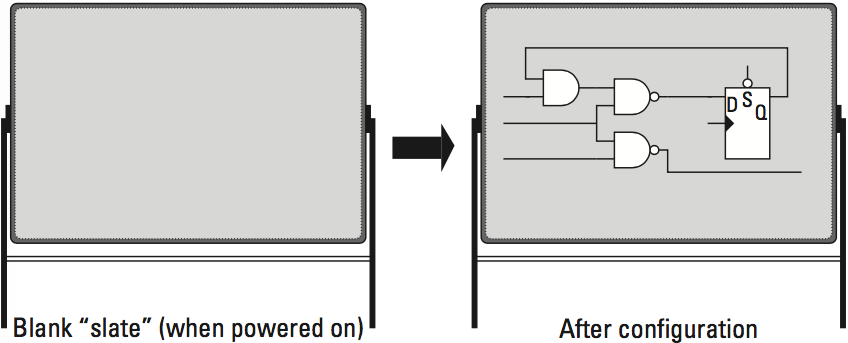
\includegraphics[width=0.75\textwidth]{img/rt-board.png}
		\caption{Ilustração em alto nível do funcionamento interno do FPGA. Fonte: \cite{Sass2010}.}
		\label{fig:rt-board}
	\end{figure}

	A seguir, será descrito a tecnologia que consiste os \hardwares\ reconfiguráveis, em especial o FPGA, e as respectivas linguagens de descrição de \hardware.

%\subsection{Sua Tecnologia}
   % PLD
   %Para introduzir alguns conceitos, é importante destacar o que são os dispositivos lógicos programáveis (PLDs, do inglês \textit{Programable Logic Devices}).
   %Às vezes chamados de dispositivos lógico programáveis em campo (FPLD, do inglês \textit{Field-Programmable Logic Device}), podem ser adaptados para criar muitos dispositivos digitais, desde simples portas lógicas até estruturas complexas.
   %\citet{tocci2003sistemas, Plessl2003} dizem que com um investimento de capital pequeno, qualquer empresa pode comprar os \softwares\ de desenvolvimento e \hardware\ necessário para programar PLDs para seus projetos digitais.
   %De modo geral, os PLDs são descritos como pertencendo a três tipo diferentes sendo eles os dispositivos lógicos programáveis simples (SPLD), dispositivos lógicos programáveis complexos (CPLDs, do inglês \textit{Complex Programmable Logic Devices}) e arranjo de portas programáveis em campo (FPGA) sendo o último tipo abordado neste trabalho \citep{Brown1996}.

   %LUTS
   O FPGA, item a ser utilizado nesta pesquisa, constitui de vários módulos lógicos programáveis relativamente pequenos e independentes, interconectados para criar funções maiores.
   Cada módulo lida, normalmente, com até quatro ou cinco variáveis de entrada.
   A maioria dos FPGAs utilizam uma \textit{look-up table} (LUT) para criar as funções lógicas desejadas.
   Uma LUT funciona como uma tabela-verdade, no sentido que a saída é programada para criar a função combinacional armazenando valores verdadeiros e falsos adequado a cada combinação de entrada.
   Os recursos de roteamento de sinal programável dentro do chip tendem a ser bem variados, com extensões de caminhos diferentes disponíveis.
   Os atrasos de sinal em um projeto dependem do roteamento real de sinal selecionado pelo \software\ de programação.
   Os módulos lógicos também contêm registradores programáveis.
   Eles não são associados a nenhum pino de entrada e saída (I/O, do inglês \textit{Input and Output}).
   Em vez disso, cada pino de I/O é conectado ao bloco programável de entrada e saída que, por sua vez, é conectado aos módulos lógicos com linhas de roteamento selecionadas.

   \begin{wrapfigure}{O}{0.5\textwidth} \centering
      \vspace{-10pt}
      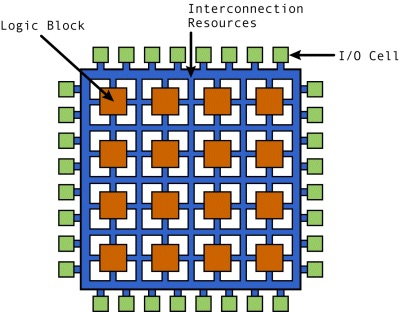
\includegraphics[width=0.5\textwidth]{img/rt-arch_fpga.jpg}
      \vspace{-15pt}
      \caption{Exemplo da arquitetura internas de um FPGA. Fonte: \url{http://www.eetimes.com/document.asp?doc_id=1274496}. Acesso: 30/05/2017.}
      \label{fig:rb-arch_fpga}
   \end{wrapfigure}

   Uma arquitetura geral simplista de FPGA é exibido na Figura~\ref{fig:rb-arch_fpga}. Nela os quadrados menores situado nas laterais são blocos de I/O que podem ser configurados para fornecer recursos de entrada, saída ou bidirecionais.
   Os quadrados maiores situados no interior são as LUTs, usados para guardar dados que entram ou saem e realizar as operações lógicas.
   Os canais que interligam os blocos entre si são estabelecidas por meio de conexões que passam pelas linhas e colunas nos canais entre esses blocos e possuem a funcionalidade de serem interconexões programáveis \citep{tocci2003sistemas}.
   %A tecnologia interna de um FPGA consiste basicamente de um arranjo de blocos lógicos, canais de roteamento para interconexão de blocos lógicos e blocos de entrada e saída de sinais em torno do circuito.
   %FPGAs baseado em SRAM (do inglês \textit{Static Random Access Memory}) utilizam células SRAM para controlar a funcionalidade de blocos lógicos e entrada e saída de sinais bem como as rotas, e pode ser reprogramado arbitrariamente em nível de circuito, muitas vezes, baixando um novo \textit{stream} de dados de configuração para o dispositivo.
   Hoje, esses dispositivos possuem milhões de portas de lógica programável, bilhões de transistores, além de outros blocos de \hardware\ dedicados dedicados como rápidas memórias embarcadas e multiplicadores de ponto-fixo tornando-o um dos circuitos integrados (CI) mais densos existente \citep{Choi2016}.

   \begin{comment}
   \begin{figure}[h] \centering
      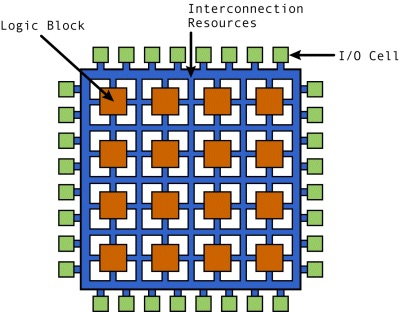
\includegraphics[width=0.5\textwidth]{img/rt-arch_fpga.jpg}
      \caption{Exemplo da arquitetura internas de um FPGA. Fonte: \url{http://www.eetimes.com/document.asp?doc_id=1274496}. Acesso: 30/05/2017.}
      \label{fig:rt-arch_fpga}
   \end{figure}
\end{comment}

   % tecnologia e energia
   Segundo \citeauthor{tocci2003sistemas}, tais maravilhas de flexibilidade de projetos digital podem fornecer uma série de opções de projeto sendo voltados para indústria e até mesmo educação.
   Ao utilizar tecnologia CMOS, o consumo de energia do chip é relativamente baixo comparado com outras tecnologias podendo ser confeccionado em nível de tensão elétrica, frequências e cargas para os sinais de I/O.
   O mercado fornece diferentes graus de velocidade de FPGA a fim de que o projetista utilize o mais adequado ao projeto.
   Entretanto, um dispositivo FPGA pode ser configurado para um número infinito de projetos e isso implica na não possibilidade de afirmar o montante de dissipação de energia para um dispositivo FPGA.
   %O \software\ Quartus II tem duas ferramentas para estimular o montante de uso de energia para uma aplicação.
   %O \textit{PowerPlay Early Power Estimator} é usado durante os estágios iniciais do projeto para estimar a magnitude de potência do dispositivo.
   Dessa forma, FPGAs são chips que podem ser programados instantaneamente para funções de qualquer circuito digital \citep{Choi2016}.

   % Importancia
   \citeauthor{tocci2003sistemas, Plessl2003} citam ainda que o motivo de PLDs estarem dominando o mercado é o fato de que, como são dispositivos programáveis, a mesma funcionalidade pode ser obtida com um circuito integrado (CI) ao invés de diversos circuitos individuais.
   Isso significa maior confiabilidade, menor espaço ocupado na placa, consumo de energia, complexidade de desenvolvimento e, geralmente, menor custo de fabricação.

   %\subsection{\textit{Hard} e \textit{Software Cores}}
   % Utilização de um processador sintético ou físico
   A unidade de processamento central (CPU, do inglês \textit{Central Processing Unit}) nesses tipos de sistema pode ser implementada em duas formas, sendo estas \textit{hard} e \textit{soft} \cores.
   O primeiro é um \core\ dedicado, ou seja, um pedaço de circuito integrado dentro (ou não) de um FPGA e o segundo é feito por meio da sintetização e mapeamento de um processador no FPGA com seus recursos lógicos, e assim, o processador é obtido por meio de \design\ e sintetização na placa por meio das portas lógicas.
   Independente da forma de projeto da CPU, o FPGA será constituído da seguinte arquitetura exibida na Figura~\ref{fig:rb-soc}, chamada de SoC FPGA (do inglês, \textit{System-on-Chip} FPGA).
   Nela, as setas representam os barramentos de comunicação entre os principais componentes.

   \begin{figure}[h] \centering
      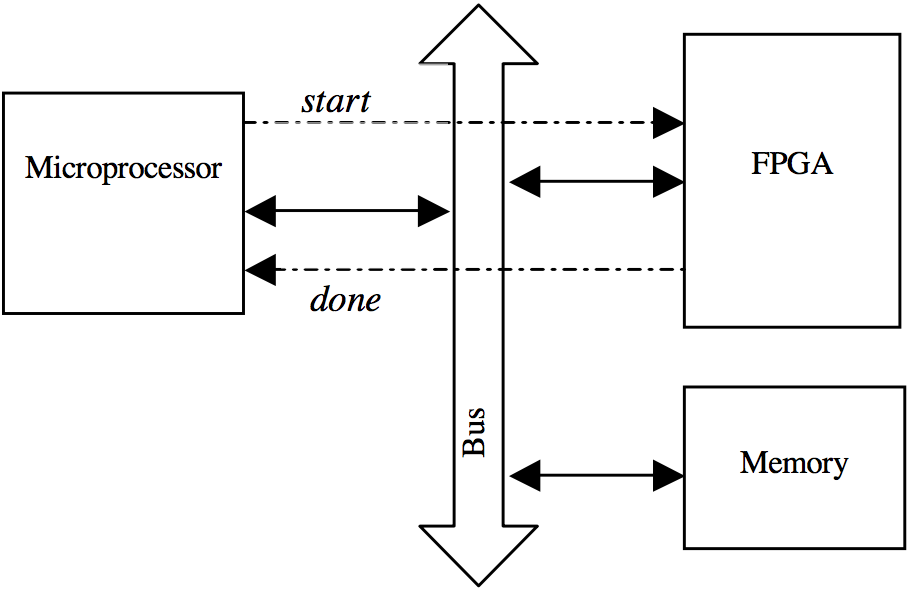
\includegraphics[width=0.6\textwidth]{img/into-soc.png}
      \caption{Visão geral de um SoC FPGA.}
      \label{fig:rb-soc}
   \end{figure}

   Cada um tipo de \core\ possui suas vantagens.
   Ao utilizar um \textit{hard} \core, é possível utilizar todos seus recursos obtendo máxima performance nas atividades executadas, a utilização de um \textit{soft} \core\ permite a extensão da arquitetura \citep{Plessl2003}.

   Um das maiores barreiras para o \design\ de projetos em FPGA é a necessidade de uso de linguagens de descrição de \hardware.
   Elas serão descritas a seguir.


	\subsection{\textit{Hardware Description Language} (HDL)}
		Linguagem de Descrição de \Hardware\ (do inglês \textit{Hardware Description Language}) é uma das classes de linguagens de computação usados para descrever formalmente um circuito eletrônico.
      Uma expressão padrão baseada em texto HDL é capaz de descrever o comportamento temporal ou a estrutura de circuito (espacial) de um sistema eletrônico.
      Sua origem veio da necessidade de documentar o comportamento do \hardware \citep{Sass2010}.

		HDL é amplamente utilizada em \design\ de \hardware\ especificando detalhes de \design\ de chip tantos chips específicos quantos os próprios FPGAs.
      Para customizar algum tipo de chip digital, HDLs especifica um modelo para um comportamento específico de um circuito antes do circuito ser projetado e construído.
      Ferramentas lógicas de sínteses são invocadas em seguida para gerar informações geométricas que são utilizadas para produzir as máscaras \textit{photolithographic}, necessárias para a fabricação do CI do projeto desenvolvido.

		A utilização de uma HDL é o primeiro passo no processo de síntese em FPGA.
      O código é entregue ao compilador lógico, chamado de ferramenta de síntese, e sua saída será carregada ao dispositivo reconfigurável.
		A propriedade única deste processo na qual fornece a lógica programável é que, com esse processo de síntese, é possível alterar o código HDL, compilá-lo e fazer sua síntese no mesmo dispositivo para testar, quantas vezes forem necessárias, sem custo adicional \citep{Smith1998}.

		Enquanto a maioria de engenheiros de \hardware\ utilizam tanto o \textit{VHDL} quanto o \textit{Verilog}, na qual possuem um nível elevado de complexidade \citep{Choi2016}, existe outras linguagens disponíveis para uso.
      Outras linguagens como \textit{SystemC}, \textit{HandelC} e \textit{Impulse} fornecem a construção de sistemas \hs\ juntos, dando ao \designer\ uma linguagem de alto nível para manuseio do projeto \citep{Sass2010}.


	\subsection{\textit{High-Level Synthesis} (HLS)}
		Sintetizador em Alto Nível (HLS, do inglês \textit{High-Level Synthesis}) são procedimentos que sintetizam códigos em alto nível para HDLs.

		Realizado uma especificação de \design\ em \software, um HLS pode reduzir os longos ciclos do processo de \design\ de \hardware\ e ainda trazer melhoria em performance e eficiência energética \citep{Choi2016}.

		As primeiras ferramentas sintetizadoras baseavam em linguagem \textit{C}, mas não houveram um sucesso em seu uso pois os engenheiros de \hardware\ acreditavam que existia uma lacuna entre o HLS e o \design\ de \hardware\ feito por humanos.
      A justificativa era que as ferramentas HLS não exploravam profundamente o recurso de paralelismo, além de que, para os engenheiros de \software\ HLS continua sendo uma dificuldade já que muitas partes do projeto, como a integração do sistema, permanecem em grande parte como um processo manual.

      Existem várias ferramentas para geração automática de código descritivo de \hardware.
      Ferramentas como o \textit{framework} LegUp e OpenCL \citep{Trevett2008} possuem o propósito de entregar um bom HLS além de tentar amenizar esses problemas de projetos.


      \subsubsection{LegUp High-Level Synthesis}
         LegUp é uma ferramenta que permite a utilização de técnicas de \software\ para implementação de \design\ de \hardware.
         Com o \textit{framework} LegUp, é possível utilizar um programa padrão  C como entrada e automaticamente compila o programa para dispositivos FPGA.

         É possível gerar procedimentos totalmente dispostos em \hardware\ e outros híbridos na qual é utiliza-se de \textit{soft} processadores, utilizando de um MIPS, e também gerando códigos para \textit{hard} processador que utiliza circuitos ARM disponibilizados em FPGAs SoCs pela Altera sendo tais gerações usufruindo de aceleradores que comunicam por meio de interface de barramentos padronizados \citep{Canis2011}.
         Possui também um \textit{framework} para \textit{debug} e verificação de HLS \citep{Fort2014}.

      \subsubsection{OpenCL}
         OpenCL é um padrão que oferece uma API comum para execução de programas em sistemas compostos por diferentes tipos de dispositivos computacionais tal como processadores \textit{multicores}, GPUs ou outros aceleradores.

         Este padrão utiliza de coprocessadores como meio para operações aritméticas intensivas paralelas e com isso é possível realizar realizar uma computação heterogênea paralela em nível de tarefas e dados, nos vários dispositivos disponíveis hoje pelo mercado criando um novo nível de infraestrutura computacional paralela.

         O OpenCL provê uma abstração fácil de uso e um amplo conjunto de APIs de programação baseada no sucesso obtido pelo CUDA (do inglês, \textit{Compute Unified Device Architecture}) e outros ferramentas de programação.
         Ele define um \core\ funcional que todos os dispositivos suportam incluindo uma mecanismo de extensão que permite os fabricantes exponham recursos de \hardware\ exclusivos e interfaces de programação experimentais para benefícios dos desenvolvedores de aplicações.

         De forma geral, um programa em OpenCL é executado num dispositivo computacional na qual os dispositivos podem conter um ou mais unidades computacionais (ou seja, \cores) na qual são compostas de um ou mais elementos de processamento SIMD (do inglês, \textit{single-instruction multiple-data}) \citep{Stone2010}.
         Como é possível visualizar na Figura \ref{fig:opencl}, levando para o ambiente de FPGAs, existe um \textit{host} que executa em um processador \textit{soft} ou \textit{hard} o \textit{ Runtime Environment} que fica responsável por controlar todos seus dispositivos.
         Cada dispositivo conectado ao \textit{host} pode conter vários \textit{processing elements} que por sua vez pode conter vários \textit{compute unit}.
         %De termos gerais, podemos associar com os conhecimentos de \software\ sendoos \textit{compute units} como \textit{threads}, \textit{processing elements} como \cores\ e os dispositivos como \textit{clusters}, sendo estes podendo ser heterogêneos.

         \begin{figure}[h] \centering
            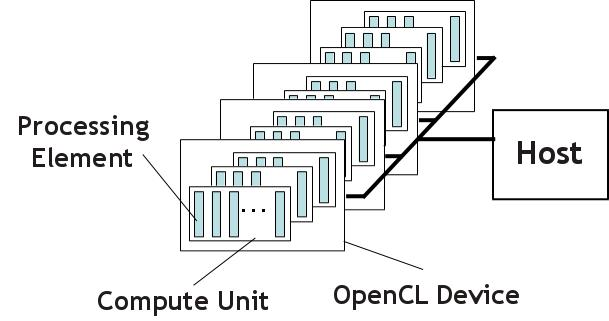
\includegraphics[width=0.7\textwidth]{img/opencl.jpg}
            \caption{Sistema hierárquico de um projeto em OpenCL. Fonte: \url{https://handsonopencl.github.io/} Acessado em: 07/08/2017.}
            \label{fig:opencl}
         \end{figure}

         Todos os aceleradores descritos neste relatório, podem ser associados com a sintetização dos procedimentos de instruções no FPGA \citep{Shagrithaya2013, Czajkowski2012}.

   		Para prover um melhor suporte para o paralelismo em \hardware, utilizaram de bibliotecas \textit{multi-threads} como a \textit{Pthread} \citep{Barney2009}, \textit{OpenMP} \citep{openmp} para criar aceleradores em \hardwares paralelos.

         É investigado otimizações em memória e arquitetura de sistema provendo melhorias em performance de circuito, área, utilizando uma abordagem do padrão produtor-consumidor para inferir circuito de transmissão em \hardware.

   \begin{comment}
   \section{Beagle Bone Black}
      Segundo \citet{Richardson2013}, além de um microcontrolador, o Beagle Bone Black é úm computador completo no qual possui suporte a sistemas como Linux Embarcado e Android, possuindo todos os componentes eletrônicos necessários para o seu funcionamento numa única placa impressa.
      Ao utilizar um sistema operacional embarcado, a placa torna-se hábil para suportar \textit{drivers} como periféricos USB e adaptadores podendo então ser adicionados módulos como câmera para captura de imagens e quaisquer outros adaptadores.

      Diferente de um típico microcontrolador que possem processadores de 8-bits, o Beagle Black Bone é capaz de compartilhar em seus processamentos em tarefas e programas, executados simultaneamente, criando um poder de processamento maior do que outros controladores sem o \textit{trade-off} do espaço\textit{die}.


      Este equipamento é voltado tanto para iniciantes com foco em aprendizagem no mundo de microcontroladores e sistemas embarcados, quanto usuários com conhecimentos avançados a fim de produzir produtos para fins mercadológicos.

      O autor \citet{Richardson2013} cita ainda que, ao comparar o Beagle Bone Black com o Raspberry Pi, o primeiro se destaca no fato de ser um produto com as características mais adequadas para fins profissionais, ou seja desenvolvimento de sistemas embarcados para projeto de produtos, o que não acontece nos dispositivos Raspberry Pi. Esses, por sua vez, possui o propósito de ser simples e didático, sendo seu \hardware\ e sistema voltados para tal.
\end{comment}


\section{\Profile} \label{sec:profile}
	%\begin{comment}
	%\end{comment}

		\Profile\ é uma procedimento para auxiliar o usuário a coletar informações do \software\ em tempo de execução.
      Existem vários programas diferentes para adquirir essas informações e podem ser distinguidos em duas categorias.
      A primeira é aqueles que apresentam a quantidade de declarações e invocações de rotinas, e aqueles que exibem informações de tempo de declarações e rotinas \citep{nemeth2004manual}. Um exemplo de saída é exibida a seguir.

{ \footnotesize
      \begin{verbatim}
Flat profile:

Each sample counts as 0.01 seconds.
  %   cumulative   self              self     total
 time   seconds   seconds    calls  ms/call  ms/call  name
 33.34      0.02     0.02     7208     0.00     0.00  open
 16.67      0.03     0.01      244     0.04     0.12  offtime
 16.67      0.04     0.01        8     1.25     1.25  memccpy
 16.67      0.05     0.01        7     1.43     1.43  write
 16.67      0.06     0.01                             mcount
  0.00      0.06     0.00      236     0.00     0.00  tzset
  0.00      0.06     0.00      192     0.00     0.00  tolower
  0.00      0.06     0.00       47     0.00     0.00  strlen
  0.00      0.06     0.00       45     0.00     0.00  strchr
      \end{verbatim}
      \vspace{-3em}
}

      \begin{wrapfigure}{o}{0.56\textwidth} \centering
         %\vspace{15pt}
         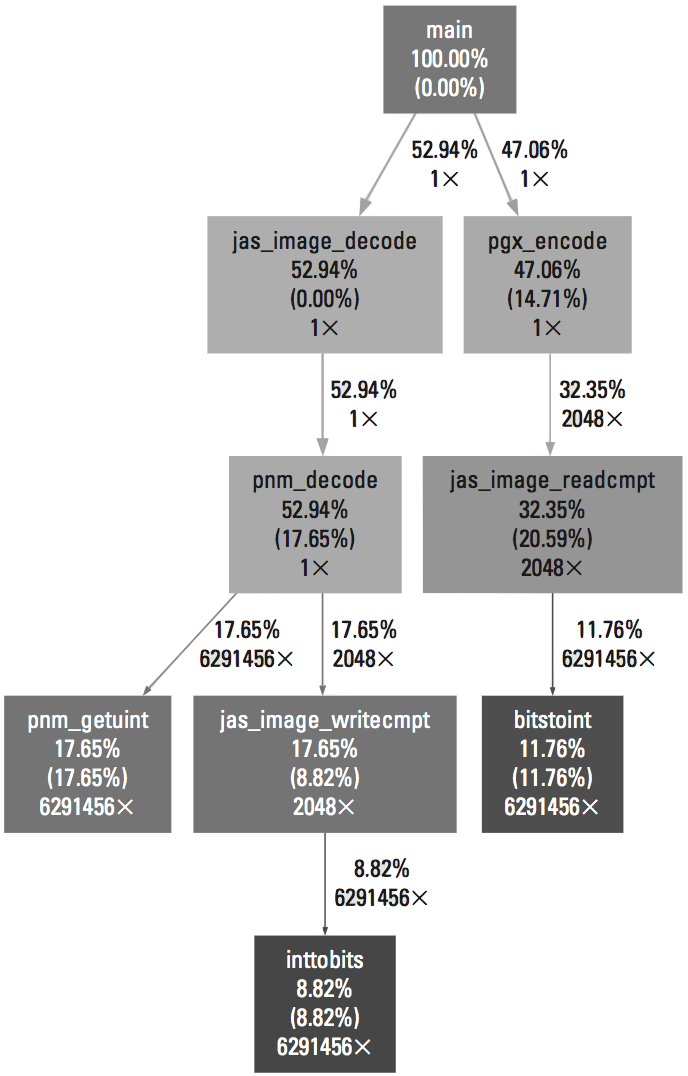
\includegraphics[width=0.48\textwidth]{img/f4-1-2.png}
         %\vspace{-1em}
         \caption{\Profile\ da codificação de imagem em formato JPEG. Fonte: \cite{Sass2010}. \vspace{-0em} }
         %\vspace{-3em}
         \label{fig:profile}
      \end{wrapfigure}

      A Figura \ref{fig:profile} exibe um exemplo gráfico de \profile\ de \software\ em um codificador de imagem em formato JPEG.
      O processo é feito ao colocar o \software\ referencial (programa a ser coletado) como entrada representativa na ferramenta e a coleta é realizada em várias partes da aplicação ao longo de sua execução neste.
		Uma das técnicas do \profile\ de mensurar uma aplicação é na realização de interrupções periódica no programa e amostrar o seu \textit{program counter}.
      Dessa forma, é possível utilizar um histograma para contar quando um programa é interrompido em um endereço particular e a partir dessa informação, calcular a fração aproximada do tempo total de execução gasto em suas partes.
      Distribuições GNU/Linux possuem a ferramenta \texttt{gprof} na qual avalia procedimentos enviados por parâmetro, realizando o cálculo de tais informações de \software\ \citep{Graham1982}.





\section{Sistemas Computacionais \Wearables}
	% Introdução histórica e geral
	Sistemas computacionais \wearables\ são sistemas que, com a possibilidade de ter um computador acoplado ao corpo, proporciona ao usuário um nível superior de informações contextualizadas dentro de um ambiente interativo \citep{Amorim2017}.

   Com a tecnologia digital constantemente melhorando à medida que a informação se torna sem-fio, os avanços demandaram mais fatores móveis e \wearable\ de produtos que possuem acesso à informação.
   Segundo \cite{Gemperle1998}, um produto que é \wearable, deveria ter sua `\textit{wearability}' sendo este definido como a interação entre o corpo humano e o objeto \textit{wearable} estendendo ao corpo em movimento.

	\begin{wrapfigure}{O}{0.5\textwidth} \centering
    	  \vspace{-10pt}
		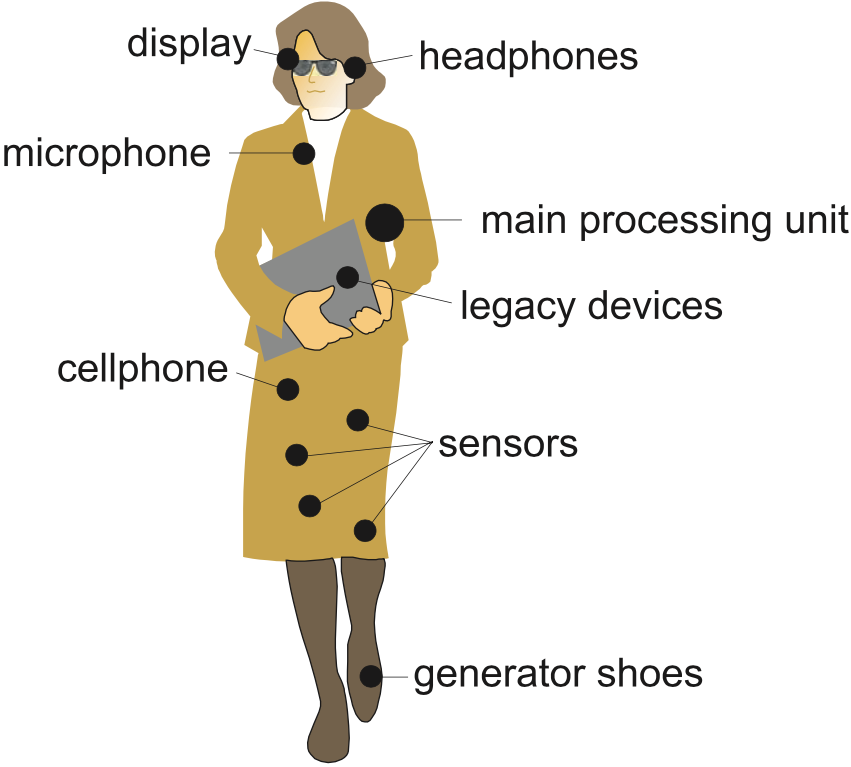
\includegraphics[width=0.5\textwidth]{img/into-wearable2.png}
        \vspace{-10pt}
		\caption{Exemplificação de alguns tipos de dispositivos \wearables. Fonte: \citet{Plessl2003}. \vspace{-15pt}}
		\label{fig:into-wearable}
	\end{wrapfigure}

	%\citep{Plessl2003}
	Devido ao movimento de seus usuários, um computador \wearable\ é embutido em um ambiente \mobile\ e necessita-se da interação com o ambiente ao seu redor.
	Como é exibido na Figura \ref{fig:into-wearable}, um sistema \wearable\ pode ser composto por um conjunto de nós distribuídos e uma rede de comunicação centralizada num módulo principal, sendo possível determinar, por exemplo, a geração de eletricidade por meio de geradores \textit{piezo-electric} integrados aos sapatos, energizando uma parte do sistema \wearable\ com o caminhar do usuário \citep{Kymissis1998} ou a ação do usuário por meio de acelerômetros \citep{VanLaerhoven2002, Kern2002}.

	Com a distribuição espacial dos módulos pelo corpo, a comunicação torna-se um item importante em termos consumo de energia \citep{Kymissis1998}.
   A rede de comunicação é uma mistura de conexões cabeadas e sem-fios.
   Para dispositivos \wearables, a comunicação sem-fio é a tecnologia predominante por causa da necessidade de mobilidade \citep{Plessl2003}.

	A introdução desses sistemas no ambiente de pesquisa não é nova como é reportado por \citet{Sutherland1968}, \citet{Mann1996} e \citet{Mann1997}.
   Entretanto, a aplicação desses dispositivos, depende diretamente da miniaturização dos componentes eletrônicos.
   Esse fenômeno fica claro ao perceber o crescente espaço ganho pelos \textit{smartwatches}, \textit{fitness trackers}, óculos, equipamentos de realidade virtual e aumentada e muitos outros nas indústrias e nas atividades pessoais de usuários.
   Com esses novos dispositivos embarcados de propósito geral miniaturizados, aumenta-se a sua atração devido à fácil disponibilidade dos dispositivos, baixo preço e ferramentas de desenvolvimento disponíveis para desenvolvimento de aplicações específicas incluindo compiladores e sistemas operacionais para tal, mas não são otimizados para uso \wearable.
	Isso pois, como \citeauthor{Plessl2003} cita, muitos dos sistemas \wearables\ construídos possuíam características diferentes de componentes que prestam auxílio à tarefas pessoais de usuários, citados anteriormente.
	Exemplos são o uso dados de teclados ou canetas para entrada de dados ou um \textit{display} LCD, na qual contradiz com o paradigma de operações \textit{hands-free} e a propriedade de computação \wearable\ discreta.
	Sistemas de computação distribuídos no corpo construídos a partir desses equipamentos interativos são altamente ineficientes devido à falta de especialização de componentes individuais de propósito específico.
	Dessa forma, a computação \wearable, seguindo esse conceitos, se define muito bem como um subconjunto de sistemas embutidos.

	% Característica de um dispositivo wearable
	\subsection{Característica de um \Wearable}
		Entendido a localização de sistemas \wearable\ sobre sistemas computacionais, a caracterização de um dispositivo \wearable\ é feita acordando as classificações pré-estabelecidas em relação à suas funcionalidades e requisitos de \hardware.
      O mercado possui um número considerável de dispositivos \wearables\ que são utilizados em inúmeras áreas, e mesmo que cada equipamento separado tenha suas próprias características, muitas soluções em \hardware\ compartilham uma arquitetura e organização interna de recursos implementados comum.
		Esses detalhes também podem ser expandidos às características relativas à recursos de sistemas operacionais, no qual dispositivos \wearables\ podem ser classificados além de seus componentes de \hardware\ internos como suas funções de performance \citep{Delabrida2016, Amorim2017}, como representado pela Figura \ref{fig:classification}.

		\begin{figure}[h] \centering
			\vspace{-5pt}
			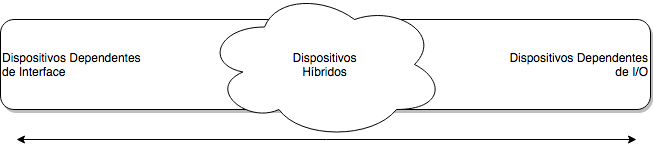
\includegraphics[width=0.9\textwidth]{img/rt-gradiente.png}
			%\vspace{-10pt}
			\caption{Classificação de sistemas \wearables. De um extremo existe os dispositivos dependentes de interfaces de usuário e do outro os dependentes de entrada e saída de sinais enquanto entre eles, a gama de combinações possíveis. Fonte: Adaptado de \citep{Amorim2017}.}
			\label{fig:classification}
		\end{figure}

		De um lado desta gama de dispositivos existem os \emph{dispositivos dependentes de interfaces de usuário} que possuem alta dependência com operações interfaces gráficas, provendo respostas sobre as interações do usuário.
      Esses dispositivos focam principalmente em tarefas para renderização em \textit{displays} como por exemplo equipamentos de realidade virtual e aumentada para implementação de objetos tridimensionais.
      %
		De outro lado, existem os \emph{dispositivos dependentes de entrada e saída de sinais}. Esses dispositivos atuam principalmente com o estímulo por algum dado oriundo de outro dispositivo ou do ambiente assim entregue à nuvem respeitando restrições de tempo real.
      Isso se da pela utilização de sensores acoplados ao dispositivo que podem exigir uma boa vazão de dados e pequena latência como são os monitores de atividade remota, situação na qual cria-se o ambiente perfeito para o termo conhecido por IoT (do inglês \textit{Internet of Things}).

		Entre dispositivos dependentes de interfaces de usuário e de entrada e saída de sinais existe os híbridos. São dispositivos que utilizam recursos de ambos os extremos citados.
      Dispositivos como \textit{smartwatches} e \textit{fitness trackers} são exemplos de tais dispositivos híbridos no qual possuem restrições de equalização à prioridade dada pelo dispositivo para ambas as operações de interface e sinais.

		A separação dos conceitos computação \wearable\ e IoT ainda não estão claros segundo a bibliografia.
      Sistemas operacionais de propósito específico para ambientes \wearable\ são comumente focado em um único tipo de seguimento de produto como os \textit{smartwatches}, sendo que proporciona aos desenvolvedores um meio para sua aplicação final além de entregar um produto de alta qualidade.
      Também, atualmente, não existe nenhum sistema que satisfaça todos os requisitos apresentados \citep{Amorim2017}.

		Já \citet{Jozwiak2017} caracteriza um sistema \wearable\ como um sistema \textit{cyber}-físico\footnote{Sendo \textit{cyber-} uma combinação dos termos `computador', `rede de computadores' ou `realidade virtual' com um segundo termo, no caso o `físico' oriundo de circuitos.} móvel autônomo.
      São sistemas que podem ter mobilidade inerente ou poder ser transportado para outro sistema, industrial ou natural (incluindo humanos), sendo autônomos em termos de funcionalidade.
      Podem ser utilizados para aplicações de consumidores (computação móvel), extensões ou reposições de capacidades humanas, sistemas sociais (\textit{health-care} inteligente), automotivo, industrial (monitoramento) e aplicações comerciais como realidade aumentada para informações turísticas.
		Eles representam uma grande parte da heterogeneidade de sistemas embarcados, cobrindo muitos campos e tipos de aplicações que vão desde um dispositivo inteligente integrado à roupa, focado no campo de computação \textit{mobile} pessoal, até indústrias como dispositivos de segurança. % \citep{Jozwiak2017}.
      Esses dispositivos podem também trabalhar de forma colaborativa com \textit{smartphones}, redes e outros sistemas criando um sistema mais complexo.

		Segundo \citet{VanLaerhoven2002}, a distribuição de elementos computacionais, como sensores, em objetos mundanos em nosso cotidiano se adéqua à pesquisa denominada por computação ubíqua.
      Isso implica também que computação \wearable\ também não foge deste arcabouço, uma vez que superfícies de roupas são uma plataforma de suporte ideal para uma grande quantidade de sensores (desde que sejam miniaturizados para que eles não obstruam o usuário).
		Essa restrição de tamanho geralmente significa que a própria qualidade do equipamento também está comprometida, o que leva ao conceito de muitos atuadores e sensores simplistas.

		Sendo sistemas \wearables\ uma subclasse de sistemas embutidos, estão sujeitos à várias restrições de \design, sendo elas performance em multi-nós, gasto energético consciente e alta flexibilidade \citep{Plessl2003}:

     \begin{description}
       	\item [Performance de multi-nós:] Requer uma performance base fixa para tarefas que não mostram altas demandas computacionais nem restrições de tempo rigorosa.
            Sistemas \wearables\ executam rajadas de tarefas de computação intensiva que consideram restrições de tempo-real.
            Não realizando as tarefas, o sistema torna-se inaplicável.

		   \item [Gasto energético consciente:] É essencial em sistema deve-se manter ativo e funcional num certo período de tempo.
            O \design\ do gasto de energia conduz inúmeros desafios como gerenciamento computacional energético eficiente e energização dinâmica.

            Diferenciando os termos de baixo custo de energia e eficiência energético, o consumo de energia é mensurado pela divisão da dissipação energética pelo tempo mensurado.
            %
            A eficiência energética relaciona o total de energia necessário para computar uma tarefa específica sendo o desafio a construção de um \design\ na qual possui-se alta eficiência energética para um dado conjunto de tarefas.
            O procedimento dinâmico de energização consiste na tarefa de associar determinada tarefa para o componente mais eficiente (energeticamente falando) disponível e forçar todos os outros não utilizados pelo sistema a serem postos em modo de economia de energia ou desligá-los quando apropriadamente.

   		\item [Flexibilidade:] Quando menciona-se sobre alta flexibilidade, é considerado o fato de que o dispositivo será utilizado em situações altamente dinâmicas.
            Isso fica claro na necessidade na qual os requisitos de aplicação variam de acordo com as escolhas do usuário, mas também com o contexto e local utilizado.
            Outro, é no fato de que o usuário troca de roupas constantemente e com isso os dispositivos devem ter a capacidade de serem acoplados e removidos, neste caso.
            Isso além de critérios como confiabilidade, disponibilidade e fatores dependentes de sua forma como volume e peso.
     \end{description}

		Dessa forma, pode-se estabelecer que os requisitos flexíveis em um sistema \wearable\ demanda um sistema de computação programável de propósito geral, enquanto os requisitos de alta performance e consumo de energia consciente demandam um sistema computacional especializado.
      Assim, como meio para solução desses problemas, \citeauthor{Plessl2003} utilizaram-se de um \hardware\ reconfigurável para incorporar ao sistema.
      O trabalho exibe um sistema \wearables\ compreendendo de um processador de até médio porte em termos de processamento e módulos reconfiguráveis.
		A utilização de \hardware\ reconfigurável nos permite alcançar alto processamento com maior eficiência energética em relação à processadores para tarefas de computação intensiva em tempo real.

	%!TEX root = ../main_text.tex
\chapter{Trabalhos Relacionados} \label{chap:relacionados}

	%O particionamento \hs\ encontra-se em duas principais bordagens sendo essas algoritmos para otimização de escolhas de particionamento e uso de recursos de determinada aplicação e o particionamento para sistemas embutidos.

	%not embedded
	O particionamento de forma geral é um problema de otimização na qual vários autores utilizam métodos para auxiliar na decisão de cada componente do \design\ referencial de \software. 
   Utiliza-se tanto processos manuais quanto algoritmos exatos ou heurísticos \citep{Arato2005}.

	\begin{wrapfigure}{r}{0.4\textwidth} \centering
    	\vspace{-20pt}
		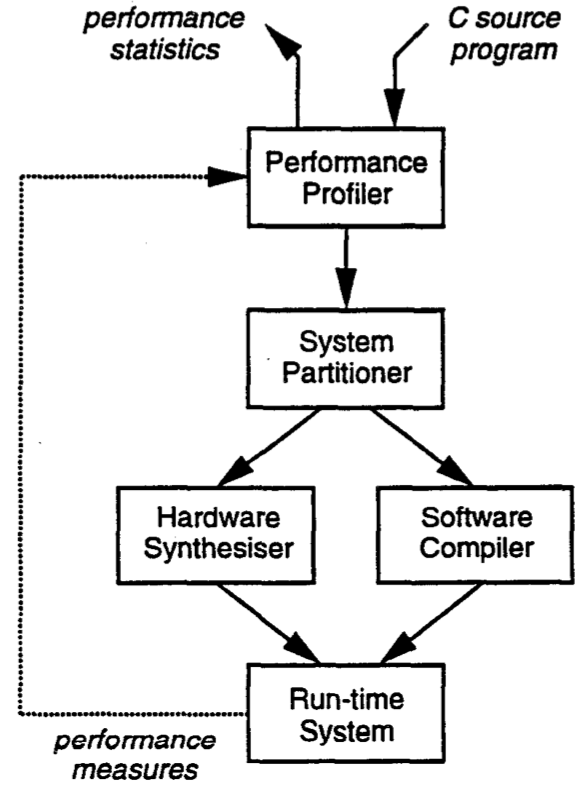
\includegraphics[width=0.4\textwidth]{img/rt-edwards_method.png}
        \vspace{-10pt}
		\caption{Metodologia de \codesign. Fonte: \citet{Edwards1994}.}
		\label{fig:tr-edwards_method}
	\end{wrapfigure}

   Os autores \citet{Edwards1994} utilizam do particionamento para aprimorar a performance do seu \software. 
   Em seu trabalho, realiza-se a tentativa de tratar regiões críticas da aplicação na qual uma solução em \software\ não pode chegar à restrições de performance requeridas e uma solução em \hardware\ deve ser encontrada, ou a performance total pode ser acelerada pela implementação de uma região crítica em \hardware.
   Apresenta-se uma metodologia para desenvolvimento \codesign\ no qual consiste na construção do código de uma aplicação em \textit{C} e as regiões críticas são identificadas e particionadas. 
   Feito isso realizar-se mensurações do projeto e uma nova verificação de particionamento é realizada, como é exibido na Figura \ref{fig:tr-edwards_method}.
   Utiliza-se também de um FPGA para as mensuras de performance e a propriedade de reconfiguração para novos testes em \hardware.
   
   Já o trabalho de \citet{Stitt2003} procura uma abordagem utilizando métodos de otimização de \software\ dinâmicos, introduzindo a primeira abordagem para particionamento de \hs\ dinâmico.
   O processo consiste na detecção da região de \software\ mais frequentemente executada e reimplementa-a em \hardware\ de FPGA.
   Afirmam que a utilização de particionamento dinâmico trás uma série de vantagens comparado com abordagens tradicionais manuais.
   
   Existem vários trabalhos que propuseram algoritmos exatos baseados em estratégias \textit{branch-and-Bound} \citep{Jigang2004, Mann2007, Strachacki2008}, programação dinâmica \citep{Madsen1997, Wu2006} e linear inteira (ILP, do inglês \textit{integer linear programming}) \citep{Niemann1997}.
   
   \citet{Nematbakhsh_theeffect} parte para o exame da relação entre o \textit{footprint} gerado para o FPGA e o \speedup\ do \software\ na situação na qual um FPGA é utilizado para a implementação de \textit{loops} e sub-rotinas críticas.
   Como utilizam uma abordagem direta, utilizaram de ferramentas protótipos e comerciais como \textit{Synopys' Nimble Compiler} e \textit{Proceler}, para a facilitação do processo.
   
   Abordagens mais recentes como a de \citet{Yan2017} parte da otimização \textit{position disturbed particle swarm} com otimização invasiva de \textit{weed} como o método de particionamento \hs.
   
   \citet{Wang2016} citam que o particionamento depende da exploração de caracterização, estimação e \design\ espacial das métricas de custo e performance sistêmica. 
   É também mencionado que o \codesign\ nos dias de hoje é tão complexo que a simplificação do particionamento só para duas partes não é suficiente para a representação do problema como um todo. 
   Sobre essa crítica, dissertam sobre a inclusão de parâmetros chave de \design\ e uso de recursos que deveriam ser incorporados à modelagem do sistema e dessa forma, o trabalho proposto visa considerar a modelagem de incerteza para particionamento de sistemas com um conjunto melhorado de parâmetros para compartilhamento de recursos \hs.
   Esse terceiro item a ser considerado ao problema de particionamento podem ser definidos em três tipos, sendo esses: 
   \textit{a)} o conjunto de recursos necessários para particionar uma dada tarefa (sendo esses RAM, ROM, DPS, blocos IP do inglês, \textit{intelectual propriety}, entre outros); 
   \textit{b)} possuem vários parâmetros de configurações que provê diferentes \textit{trade-off} entre recursos e performances como por exemplo circuitos de multiplicações/divisões que podem ser sintetizados sequencialmente (pouca área e lento) ou combinatório\footnote{Por \textit{unrolling}, técnica de otimização de código no qual tenta reduzir ou eliminar as iterações de determinado \textit{loop} do código.} (muita área e rápido); 
   \textit{c)} a dificuldade da mensura de desempenho e impacto no uso de recursos em várias configurações de partição com precisão precisando ter em mente a partição com a natureza incerta dessas estimativas não precisas.
   A teoria da incerteza é uma abordagem que é um sistema matemático que é designado para modelar a indeterminação ao invés do uso da teoria da probabilidade. 
   Isso pois, quanto tem-se muitas amostras de uma quantidade indeterminada, seria significativo a utilização da teoria de probabilidade ou \textit{fuzzy} pela propriedade de serem contínuas entre o intervalo 0 (zero) à 1 (um). 
   Entretanto, se não possui-se amostras suficientes para a estimação de uma distribuição de probabilidade, utiliza-se do conhecimento do domínio para avaliação do grau de crença de que cada evento indeterminado acontecerá, no caso, aplicado pela teoria da incerteza. 
   E a teoria da incerteza é um ramo da matemática axiomática para modelagem de graus de crença, de modo geral.
   
   Como outro trabalho recente que aborda o particionamento, \cite{Choi2016} descreve um \textit{framework} chamado LegUp.
   Com essa ferramenta é possível compilar um \software\ e suas \textit{threads} gerando um sistema \textit{hardware-only} ou também um sistema híbrido particionado paralelo utilizando aceleradores, gerando também todos os itens necessários para tal como memórias sintetizadas e sistemas de interconexões.
   Utilizam duas técnicas de descrição de paralelismo em \software\ sendo elas a \textit{Pthreads} e a \textit{OpenMP} sendo a primeira permite a sintetização de funções operando concorrentemente em \hardware\ com aceleradores, e a segunda usada para gerar os próprios aceleradores executados concorrentemente em um sistema de compartilhamento de memória.
   Afirmam também que a sua ferramenta produz HDL de alta performance que pode ser comparado com circuitos que são gerados por ferramentas HLS comerciais. 
   Os resultados obtidos pelos cientistas \cite{Canis2011} mostraram que a ferramenta consegue gerar produtos tão bons quantos ferramentas HLS comerciais.
   
   Entretanto, além de todo arcabouço de algoritmos para escolhas para sistemas de propósito geral tal como os citados, existe ainda uma linha de pesquisa específica do problema na qual trata-se do particionamento em sistemas embutidos.
   
   
   % Embedded
   O desenvolvimento para sistemas \hs\ participativo para sistemas embutidos ou microcontroladores já é pesquisado amplamente como os trabalhos de \citeauthor{Ernst1993, Gupta1995, Hardt1995, Gajski1994, Bolsens1997}, publicados na década de 90.
   \citet{Mei2000} em seu trabalho, descreve um particionamento de \hs\ além de uma abordagem de escalonamento para sistemas embutidos dinamicamente reconfiguráveis (DRESs, do inglês \textit{dynamically reconfigurable embedded systems}) no qual possuem como projeto um processador de propósito geral junto com um FPGA sendo este reconfigurável em tempo de execução para reduzir custos.
   Dessa forma, seu trabalho consiste numa análise de tempo de configuração e, como contribuição, a análise do tempo de reconfiguração parcial do FPGA.
   %Com a adição da reconfiguração parcial de \hardware, o escalonamento no FPGA torna-se um problema de alocação restrita, enquanto o escalonamento em circuitos integrados de aplicação específica (ASICs, do inglês \textit{application-specific integrated circuits}) é um problema de serialização.
   Para o escalonamento, \citeauthor{Mei2000} utiliza um método baseado na heurística do algoritmo genético (GA, do inglês \textit{genetic algorithm}) e num algoritmo de escalonamento de lista com melhorias.
   O escalonador desenvolvido atua como uma sub-rotina do algoritmo de particionamento. 
   Ele é invocado no passo \textit{evolution} do GA. 
   Além do escalonamento já conhecido em processador e barramento sequenciais determinando a ordem e tempo início de execução, o algoritmo também deve fazer o escalonamento no FPGA.
   Porém, não só determinando o tempo de início da tarefa, mas sim sua posição no FPGA respeitando as restrições de recursos e precedentes, tornando assim o problema uma abordagem ao problema de alocação restrita.
   
   Já \citet{Arato2003} descreve algumas versões diferentes do problema de particionamento, correspondendo à sistemas de tempo-real e custo restringido respectivamente, fornecendo análise matemática formal para o problema, provando que são problemas $ \mathcal{NP} $-difícil. 
   Apresentaram uma abordagem baseada na programação linear inteira resolvendo o problema de forma otimizada, mesmo para sistemas de grande porte, além de outra abordagem utilizando a heurística GA na qual encontrar soluções próximas ao ótimo global para sistemas largos.
   
   \citeauthor{Mann2007}, em \citeyear{Mann2007}, descreveram uma primeira tentativa para um algoritmo exato, não heurístico, para o problema de particionamento. 
   Utilizam um esquema na qual implementa-se a estratégia \textit{branch-and-bound} como um \textit{framework}, permitindo o incremento de outros algoritmos. 
   Em sua implementação, realizaram várias investigações para incrementar a eficiência do algoritmo, incluindo várias técnicas sendo elas: \textit{lower bounds based on LP-relaxation}, uma mecânica de inferência customizada, condições não-triviais necessárias baseadas num algoritmo \textit{minimum-cut}, e diferentes heurísticas com passos pré-otimizados. 
   O algoritmo também pode ser generalizado a fim de incluir mais de uma restrição, podendo também o \designer\ prescreva quais nós devem estar em qual nível de projeto. 
   Eles demonstram que o produto pode resolver problemas de particionamento altamente complexos em tempo razoável. 
   Citam ao final que o resultado obtido é em entorno de dez minutos mais rápido que algoritmos exatos anteriores baseados em programação linear inteira para os testes realizados.
   
   Pesquisas mais recentes como a de \citeauthor{Hassine2017}, em \citeyear{Hassine2017}, procuravam aplicar otimizações sobre o tempo de execução e gasto energético para \cores\ baseados em sistemas embarcados por meio de algoritmos de particionamento.
   O algoritmo proposto destina-se a alcançar um particionamento de grafos à procurar o melhor conjunto da relação energia e tempo de execução.
   Testado em comparação com outros algoritmos heurísticos como \textit{Simulated Annealing}, Busca Tabu e Genético, o algoritmo mostra-se ser melhor adequado para aplicações em \cores\ baseados em sistemas embarcados que necessitam do equilíbrio no \textit{tradeoff}.
   
   \citet{Trindade2016} por exemplo utiliza do GA para solucionar o problema de particionamento em sistemas embutidos. 
   Em seu trabalho, é proposto novas abordagens para o problema usando técnicas de verificação baseadas nas teorias de módulo de satisfação (SMT, do inglês \textit{satisfiability modulo theories}). 
   Apresentam um exemplo de particionamento, modelam e solucionam-o usando três diferentes técnicas sendo a principal ideia é aplicar mo método de verificação SMT ao particionamento \hs, e por fim, comparar os resultados com técnicas de otimizações tradicionais como ILP e GA.

   \citeauthor{Jozwiak2017} em seu \textit{survey} publicado em \citeyear{Jozwiak2017}, considera vários aspectos de uma aplicação embutida, bem como suas tecnologias de \design\ com foco sistemas móveis modernos e \wearables.
   É citado dois paradigmas de desenvolvimento para sistemas embutidos sobre sistema de multi-processadores heterogêneos sendo eles o paradigma de sistemas \textit{life-inspired} e sistemas \textit{quality-driven}. 
   O paradigma de sistemas \textit{life-inspired} especifica princípios básicos, características e organização funcional e estrutural de um sistema embutido por meio da analogia à vida de um organismo inteligente, além de básicas soluções de mecanismos e arquiteturas de sistemas para implementar tais princípios. 
   Já o paradigma de sistemas \textit{quality-driven} (ou seja, orientado pela qualidade) torna-se uma segunda solução para o \design\ de dispositivos que necessitam satisfazer as exigências de \textit{real-time}, baixo consumo de energia, entre outros. 
   Dessa forma, especifica-se qual a nova qualidade do sistema a ser requeria e como esta meta é obtida. 
   De forma a facilitar a compreensão, \citeauthor{Jozwiak2017} define qualidade de uma solução sistêmica proposto como o total de sua eficácia e eficiência na resolução do problema real. 
   Eficácia entende-se como o grau em que uma solução atinge seus objetivos e a eficiência o grau em que uma solução usa recursos para realizar seus objetivos e juntas determinam o grau de excelência. 
   Elas são expressas em termos de parâmetros mensuráveis, o que é necessário para implementar o design \textit{quality-driven}.
   Entretanto, é descrito ao final que, enquanto \designers\ aprenderam bastante na construção de plataformas de \hardware\ heterogêneos altamente paralelos, os métodos e ferramentas automatizadas para a sua programação e o paralelismo do algoritmo, bem como o \codesign\ coerente da arquitetura \hs\ ainda são atrasados perante à tecnologia.
      
   Por fim, verificando no espectro de \wearables, é possível ver vários trabalhos \citep{Plessl2003, Ahola2007, Abdelhedi2016, Narumi2016, Lee2015} que relacionam FPGAs com aplicação \wearable.
   Entretanto, nenhum trabalho menciona análise metodológica do problema de particionamento \hs\ para \design\ de sistemas computacionais \wearables\ e seus requisitos de funcionamento, tema tratado nesta pesquisa.


   \section{Comparativo entre os Trabalhos}      

      Fazendo uma relação entre a pesquisa proposta com os trabalhos relacionados, é possível visualizar pela Tabela~\ref{tab:comparativo_trabalhos} que, a pesquisa tem como proposta uma metodologia para o particionamento \hs\ de dispositivos \wearables\ utilizando recursos em \hardware\ reconfigurável a fim de buscar otimizações em sua performance utilizando aceleradores em \hardware.
    
   \begin{table}[h] \scriptsize
      \caption{Comparativo visual entre os principais itens tratado nos trabalhos relacionados e o trabalho aqui apresentado.}
      \label{tab:comparativo_trabalhos}
      \rowcolors{1}{lightgray}{white}
      \begin{tabularx}{\textwidth}{|X|c|c|c|X|} \hline
         \textbf{Trabalhos Relacionados} \centering & 
                                         \specialcell{\textbf{Particio-}\\\textbf{namento}} &
                                                  \specialcell[h]{\textbf{Embarcado/}\\\textbf{\Wearable}} & 
                                                                     \textbf{FPGA} & 
                                                                              \textbf{Observações Adicionais} \\ \hline \hline
                                                                             
         \citet{Edwards1994}           & \cmark & \cmark\ / \xmark & \cmark & Proposta de uma metodologia nova \\ \hline
         \citet{Stitt2003}             & \cmark & \cmark\ / \xmark & \cmark & Particionamento Dinâmico \\ \hline
         \citet{Jigang2004, Mann2007, 
         Strachacki2008}               & \cmark & \xmark\ / \xmark & \xmark & \textit{Branch-and-bound} \\ \hline
         \citet{Madsen1997, Wu2006}    & \cmark & \xmark\ / \xmark & \xmark & Prog. dinâmica \\ \hline
         \citet{Niemann1997}           & \cmark & \xmark\ / \xmark & \xmark & Prog. linear inteira \\ \hline
         \citet{Nematbakhsh_theeffect} & \cmark & \xmark\ / \xmark & \cmark & \textit{Footprint} FPGA vs. \speedup\ \software \\ \hline
         \citet{Yan2017}               & \cmark & \xmark\ / \xmark & \xmark & Otimização \textit{position disturbed particle swarm} \\ \hline
         \citet{Wang2016}              & \cmark & \cmark\ / \xmark & \cmark & Modelagem de incerteza para o particionamento \\ \hline
         \cite{Choi2016}               & \cmark & \xmark\ / \xmark & \cmark & \textit{Framework} LegUp \\ \hline
         % embedded
         \citet{Mei2000}               & \cmark & \cmark\ / \xmark & \cmark & Processador (Particionamento e escalonamento para sistemas embutidos dinamicamente reconfiguráveis com GA) \\ \hline
         \citet{Arato2003}             & \cmark & \cmark\ / \xmark & \xmark & Particionamento para RTOS e custo restringido, utiliza-se de prog. linear inteira \\ \hline
         \citet{Mann2007}              & \cmark & \cmark\ / \xmark & \xmark & \textit{Branch-and-bound} \\ \hline
         \citet{Hassine2017}           & \cmark & \cmark\ / \xmark & \xmark & Otimizações em \cores. Particionamento que visa o tempo de execução vs. gasto energético \\ \hline
         \citet{Trindade2016}          & \cmark & \cmark\ / \xmark & \xmark & Utiliza algoritmo genético \\ \hline
         \citet{Jozwiak2017}           & \cmark & \cmark\ / \xmark & \xmark & \textit{Survey} sobre particionamentos em sistemas embutidos. Classifica-os em dois paradigmas: \textit{life-inspired} \textit{quality-driven} \\ \hline
         % fpga
         \citet{Plessl2003, Ahola2007, 
         Abdelhedi2016, Narumi2016, 
         Lee2015}                      & \xmark & \cmark\ / \cmark & \cmark & Não realizam análise metodológica sobre o problema de particionamento \\  \hline \hline
         \textbf{Trabalho Proposto}    & \cmark & \cmark\ / \cmark & \cmark & \textbf{Metodologia para \wearable\ com foco em aumento de \speedup\ e controle energético} \\ \hline
       \end{tabularx}
   \end{table}

   A tabela exibe todos os trabalhos apresentados de forma a pontuar as ferramentas e os propósitos.
   Como existe muitos trabalhos que abordam sistemas embutidos, foi adicionado uma especificação na qual indica se além do foco em sistemas embarcados, o trabalho proposto também possui uma análise em sistemas \wearables.
   Há trabalhos que trabalham com o particionamento, mas sem foco em \wearables, outro que não utilizam de plataformas FPGA como meio para a obtenção de seus objetivo e outros que trabalham com \wearables\ e FPGA mas o objetivo do estudo do particionamento.
   Dessa forma, a pesquisa tende a realizar uma análise utilizando todos estes conceitos, sendo eles, o particionamento para \wearables\ utilizando plataformas FPGAs.
	\input{tex/chap-Metodologia.tex}
	%\input{tex/chap-Resultados.tex}
	%!TEX root = ../main_text.tex
%\chapter{Experimentos e Resultados} \label{chap:experimentos}

\chapter{Conclusões Parciais e Trabalho Futuro} \label{chap:conclusao}

   Neste capítulo serão descritas as conclusões parciais da pesquisa realizada até o momento e as próximas etapas a serem executadas.   

   \section{Conclusões}
      %demora da pesquisa em wearables
      Mesmo a tecnologia embarcada tenha tido um grande avanço nos últimos tempos sendo utilizada nos mais diversos fins, sistemas \wearables\ tiveram seu primeiro aparecimento em pesquisas científicas em \citeyear{Mann1996} por \citeauthor{Mann1996}.
      Isso, por causa de empecilhos tecnológicos e ferramentais como a necessidade da miniaturização, mobilidade e eficiência energética da tecnologia dos equipamentos utilizados na qual, sem tais especificações, seria inviável a utilização do \wearable.
      
      %não tem particionamento para wearables
      Existe várias pesquisas relacionadas à área de sistemas embarcados no âmbito de particionamento de \hs, inclusive utilizando FPGAs como meio.
      Entretanto, até o momento deste, não foi encontrado nenhum relato de experiências científicas sobre o particionamento para sistemas \wearables\ com utilização de recursos de \hardwares\ reconfiguráveis, tema tratado neste documento.
      
      % objetivos concluídos até então
      Objetivos realizados até o presente momento:
      
      \begin{itemize}
         \item Introdução de sistemas computacionais \wearables\ e apresentação do problema de particionamento \hs\ no âmbito de de sistemas computacionais embutidos, com foco em sistemas \wearables;
         
         \item Apresentação de:
         \begin{itemize}
            \item Principais soluções apresentadas ao logo dos anos e as utilizadas atualmente;
            \item Ferramentas HLS como LegUp e OpenCL para a geração de sistemas computacionais que usufruem de aceleradores em \hardware.
         \end{itemize}
         
         \item Apresentação da abordagem metodológica a ser utilizada para a procura da solução do problema de particionamento \hs\ apresentado.
      \end{itemize}
      
      
   \section{Trabalho Futuro}
      A seguir será apresentado os tópicos relativos às próximas etapas a serem realizadas neste trabalho.
      
      \begin{itemize}
         \item Geração de HDL, utilizando as ferramentas automatizadas quando aplicável:
         \begin{itemize}
            \item LegUp;
            \item OpenCL.
         \end{itemize}
         
      \item Realizar-se-á análises de algoritmos situados em sistemas diferentes, sendo esses:
         \begin{itemize}
            \item \textbf{Totalmente em nível de \software:} sem auxílio de qualquer acelerador como ao utilizar a plataforma Beagle Bone como sendo o sistema embarcado completo para execução em aplicações \wearables; e em
            
            \item \textbf{Híbridos:} formados de processadores e aceleradores utilizando dos recursos de dispositivos reconfiguráveis  a fim de prover maior \speedup\ utilizando recursos de \hardware.
         \end{itemize}
         
         \item A análise de desempenho será feita com os dados obtidos dos dois sistemas citados acima.
         Executando o projeto nos dois sistemas, em nível de \software\ e híbrido, é possível relacionar o ganho de desempenho realizando as operações apresentadas na Seção~\ref{sec:ganho_performance}.
                  
         
      	\item Redução do tempo de seu desenvolvimento até a disposição do produto ao mercado utilizando os recursos que o desenvolvimento com \hardware\ reconfigurável proporciona. %Wolf1994.
         \end{itemize}
      
\end{mainmatter}

%% Produce the appendices
\begin{appendices}
\begin{flushleft}

\end{flushleft}
	  \selectlanguage{brazilian}
  	%!TEX root = ../main_text.tex

\chapter{Apêndices}


\begin{comment}
\section{\Benchmarks}
\citep{Trindade2016}

% intro
Por serem um excelente mensurador de performance de aplicações e processadores, \designs\ têm feito de \benchmarks\ uma parte crítica do processo de \design\ de projetos.
Uma vez que um \benchmark\ torna-se padrão e popular em um ramo de pesquisa, cria-se então uma alta pressão em aumento de performance por otimizações \citep{Hennessy2011}.

% utilização de benchs no trabalho
% arato2005
Para a demonstração e validação da solução a ser desenvolvida, será utilizado %vários \benchmarks\ e exemplos randômicos largos.
\benchmark\ de \textit{MiBench}.
Esse \benchmark, segundo \citeauthor{Guthaus2001} foi escolhido com base em um exame e comparação de um conjunto de aplicações embarcadas representativas comercialmente com o conjunto de \benchmarks\ SPEC2000 \citep{Case1995}.
\end{comment}


\begin{comment}
Por exemplo, considerando as vogais da língua inglesa onde o universo $ U = \{a, e, i, o, u, y\} $. 
Assim, uma partição desse problema $ \mathcal{X}_a $ de $ U $ pode ser representado por


\begin{equation}
\mathcal{X}_a = \left\{\{a, e, i, o, u\}, \{y\}\right\} \label{eq:xa}
\end{equation}

e supondo que o conjunto pode ser representando por cada unidade, uma outra forma de representação pode ser


\begin{eqnarray}
\mathcal{X}_b &=& \left\{\{a\}, \{e\}, \{i\}, \{o\}, \{u\}, \{y\}\right\}
\end{eqnarray}

Sobre tais conceitos, a Partição \ref{eq:part_c} viola a Equação \ref{eq:part_form_1} e a Partição \ref{eq:part_d} viola as Equações \ref{eq:part_form_2} e \ref{eq:part_form_3}.

\begin{eqnarray}
\mathcal{X}_c &=& \left\{\{a\}, \{e\}, \{i\}, \{o\} \right\} \label{eq:part_c} \\
\mathcal{X}_d &=& \left\{\{a, e, i\}, \{i, o, u, y\}, \{\}\right\} \label{eq:part_d}
\end{eqnarray}

A Figura \ref{fig:f4-2} ilustra o $ \mathcal{X}_a $ graficamente, segundo a Partição \ref{eq:xa}.

\begin{figure}[h] \centering
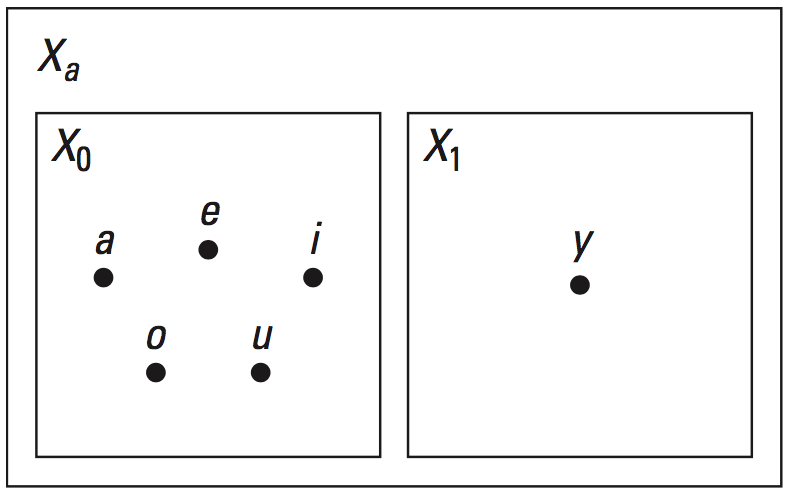
\includegraphics[width=0.5\textwidth]{img/f4-2.png}
\caption{Figura representativa do mapeamento da aplicação.}
\label{fig:f4-2}
\end{figure}
\end{comment}


%\chapter{Transferência de Estado} 

\section{Transferência de Estado} \label{chap:tranferencia}
   Segundo \citeauthor{Sass2010}, manter estado consistente sobre dispositivos FPGA e processadores é um desafio.
   Isso pois, como cada FPGA tem sua própria hierarquia de memória independente, estados são amplamente distribuídos no \design\ e há ampla variedade de interconexões entre FPGA e processadores.
   Assim, isso significa menos estados para serem transferidos e grande variedade de mecanismos disponíveis.
   Os tipos de estados serão descritos a seguir pois são requisitos para identificação de qual parte do estado da aplicação precisa ser explicitada pela comunicação processador e recurso.
   %Para entender melhor deve-se definir dois conceitos sendo eles estado afetado e preso ajudando a decidir quais partes do estado da aplicação necessitam de ser explicitamente comunicados entre processador e recurso.
   
   \begin{description}
      \item [Estado Afetado:]
      Na computação alguns estados são independentes pela construção e não precisam de ser transferidos de lugares. Retirando tais estados, restam os estados afetados.
      
      Esses, são os dados da aplicação que, durante a transferência de controle, podem ser modificados ou lidos por um recurso ou processador, necessitando de ser consistente entre todas as distribuições.
      %Estados afetados podem existir em grande escala. Principalmente quando arranjos, estruturas de dados complexas ou ponteiro estão envolvida e podem ser acessados de várias formas possíveis e geralmente não é possível saber se dois ponteiros estão apontando para um mesmo endereço.
      
      \item [Estado Preso:]
      Acontece quando parte da hierarquia de memória é compartilhada, nem todo o dado tem que ser explicitamente transferido e assim, caso todo o estado corrente esteja em memória primária (RAM) e ambos os dispositivos possuem acesso a ela, então não existe razão para a transferência explícita dos dados.
      
      Processadores modernos são construídos com quantidade significativa de memória que podem ser utilizadas como parte de estado sem a atualização da memória primária.
      Compiladores naturalmente utilizam toda a vantagem de registradores para armazenar os estados.
      
      Implementações em \hardware\ também incorporam dados ao longo do projeto e seus registradores e \textit{flip-flops} possuem valores intermediários entre ciclos de \textit{clock} dentro do projeto.
      O estado de uma aplicação é armazenado em várias partes do sistema.
      Para um recurso implementar parte de uma aplicação, precisa-se então integrar-se com parte do estado.
      
      Esse pode ser considerado mais facilitado pelo fato de que o estado está localizado em um espaço comum. Mas se um estado está localizado num registrador ou em uma cache de um processador, ele não pode ser acessado pelo sistema externo e, neste caso, o estado encontra-se preso e deve ser explicitamente transmitido pela interface.
      
      \begin{figure}[h] \centering
         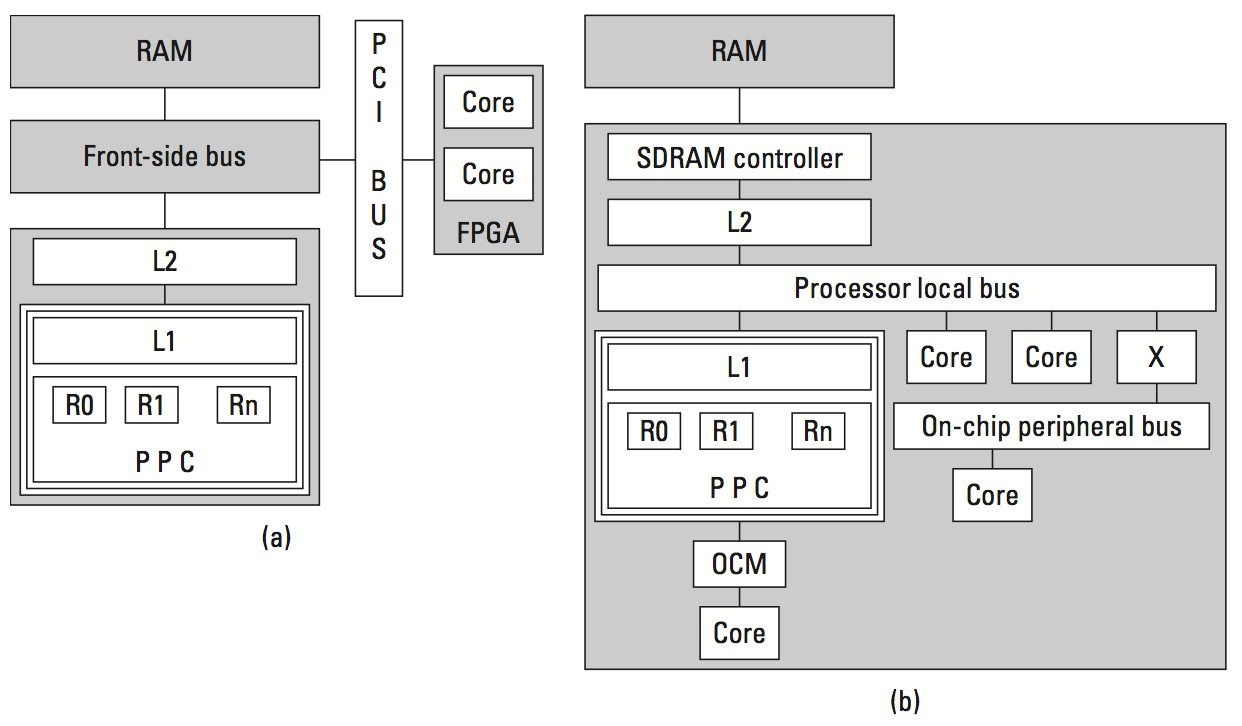
\includegraphics[width=1\textwidth]{img/f4-7.png}
         \caption{Situações na qual pode ocorrer bloqueio de estado. \textit{a)} Situação na qual existe um processador externo ao FPGA e sua memória interna é inacessível. \textit{b)} Situação onde o processador situa-se na plataforma FPGA. Fonte: \citet{Sass2010}.}
         \label{fig:4-7}
      \end{figure}
      
      Em ambos os casos mostrados na Figura \ref{fig:4-7} o FPGA (representado pelos \cores\ não possui autorização para o acesso aos registradores do processador (representados por $R_n$). Mesmo em \textit{b)} onde o processador é integrado à plataforma FPGA, não possui-se acesso sendo necessário a disponibilização manual deste.
   \end{description}
   
   
   \section{Problema de Transferência de Estado}
   Estados afetados que estão presos necessitam de ser explicitamente comunicados e esta é feita por um processo chamado \textit{marshaling}.
   Assim, será feito um \textit{Marshaling} de grupos de elementos de um estado afetado de uma aplicação em registros lógicos que são explicitamente transferidos.
   
   Tendo a premissa que o processador possui o controle inicial, tem-se quatro tipos de registros que podem ser utilizados.
   Os dois primeiros, \textit{Type-I} e \textit{Type-F}, são utilizados para iniciar e outro para finalizar a transferência de um conjunto de elementos para o recurso, respectivamente.
   Os outros dois tipos de \textit{marshal} são usados repetidamente. Um quando o recurso é invocado (\textit{Type-CI}, do inglês \textit{copy-in}), e quando é completado (\textit{Type-CO}, do inglês \textit{copy-out}).
   %Um exemplo de \textit{Type-F} é quando tem-se um \core\ que acumula um valor em uma variável global. O registro \textit{Type-F} seria utilizado para ler o valor da variável após sua última invocação.
   
   Um processo de tradução pode ser incorporado com o \textit{marshaling}, sendo o exemplo a conversão de ponto flutuante para fixo quando transferido para um recurso o que acontece também com transformações mais complexas.
   %O agrupamento de elementos é lógico pelo fato do \textit{assembly} não significar estritamente que os elementos são copiados para uma memória de locação contínua.
   
   A forma mais simples de transferir estados é copiando os registros, parando o processador enquanto o recuso processa.
   Este é chamado de \textit{push} os dados no qual transmite o dado antes da transferência do controle. Ao final, realiza-se o \textit{pulls} dos dados.
   
   
   Embora isso, uma transferência instantânea de estado não é sempre simples. Quando o estado afetado é grande mas o dado atua é pequeno, o padrão de acesso ao dado é randômico e a transferência lógica de registro é larga sendo mais vantajoso o uso de interfaces de comunicação para servir o recurso. Ou seja, utilizado quando o recurso foi designado para reduzir a latência da tarefa e a transferência do registo é pequena.
   Quando o registro lógico e o dado atual são largos, utiliza-se de padrão de acesso regula que transmite dados continuamente. É usado quando o recurso aumenta o \textit{throughput} e a redução de latência ou metas de performance não são possíveis.
   
   Isso é útil por exemplo na ordenação onde transferir um arranjo completo quando invocado é uma operação cara e desnecessária já que dependendo do algoritmo, pode-se utilizar apenas frações deste.



\section{Análise de Performance de Sistema} \label{sec:amdahl}
	A análise de performance de um sistema é definida pela Lei de \citeauthor{amdahl1967validity} de \citeyear{amdahl1967validity} relaciona o tempo gasto para executar uma tarefa com um único processador e o gasto com $j$ processadores. Nessa definição, $T_1$ representa um computador sequencial e $T_j$ um computador com $j$ núcleos. Sendo $s$ a fração relativa ao trecho estritamente serial e $q$ a fração relativa ao tempo paralelizável, tem-se as seguintes definições básicas

	\begin{eqnarray}
		T_1   & = & s + q = 1\\
		T_j & = & T_1 \times s + T_1 \times  \left(\frac{q}{j}\right)
	\end{eqnarray}

    O \textit{speedup}, cálculo do ganho da utilização de vários \cores, é obtido pela Fórmula \ref{eq:spu_init}.

	\begin{eqnarray}
		Speedup & = & \frac{T_1}{T_j} \label{eq:spu_init}
	\end{eqnarray}

	Dessa forma, realizando substituições das definições básicas na Equação \ref{eq:spu_init}, tem-se a Equação final de \speedup\ em \ref{eq:spu_fim}.

	\begin{eqnarray}
		Speedup & = & \frac{T_1}{T_j} = \frac{(s + q)}{\left(s+\frac{q}{j}\right)} = \frac{1}{\left(s+\frac{q}{j}\right)} \\
		%T(n) & = & T(1)(B + \frac{1}{n}(1 - B)) \\
		Speedup & = & \frac{1}{s + \left(\frac{1 - s}{j}\right)} \label{eq:spu_fim}
	\end{eqnarray}

	Essa equação articula os limites de um melhoramento global para uma aplicação que um simples aprimoramento pode fazer em tempo de execução.

	Generalizando a equação para incluir todo potencial de aprimoramento e métricas de performance arbitrária, pode-se caracterizar os limites como coleções de aprimoramento.
    Se esses aprimoramentos são recursos de \hardware\ e podemos antecipar o ganho requerido ganho potencial de recursos para cada recurso, então pode-se desenvolver um modelo que irá orientar ao processo de particionamento.

    Tal lei não é adequada pois:
	\begin{itemize}
		\item Visa um simples realce e não nos auxilia a selecionar um subconjunto de uma coleção de recursos potenciais;
		\item Foca somente no tempo de execução;
		\item Não visa recursos requeridos;
		\item Não visa custo de comunicações.
	\end{itemize}

	Perfis baseados em exemplos requerem representações de entrada e é uma aproximação de tempo gasto. Sem implementar todo o potencial de recursos em \hardware, pode ser difícil antecipar os recursos requeridos. Pode-se com determinação analítica calcular quantos ciclos de \textit{clock} um recurso de \hardware\ irá tomar, podendo assim calcular métricas como \speedup. Entretanto, é impossível saber quando um processo arbitrário será completado. Ao invés de prover uma solução automatizada, a solução analítica simplesmente provê um \textit{framework} para guiar um \designer\ de sistema a criar uma solução criativa.

	\subsection{Abstração e Estado}
		No contexto de desenvolvimento, um módulo é uma abstração de alguma funcionalidade em um sistema.
		A palavra abstração é definida como `operação intelectual em que um objeto de reflexão é isolado de fatores que comumente lhe estão relacionados na realidade', ou seja, no sentido amplo da palavra, significa tirar fora, extrair, remover.
		Um módulo tenha uma boa abstração terá suas interfaces e descrições mais fáceis de serem compreendidas, entretanto isso torna sua implementação mais complexa.
		Uma boa abstração capta todas características importantes de algo criando assim uma organização e dessa forma, uma representação rica em informação pode não ser tão relevante\todo{rever}.
		Em contra partida, caso seja feito uma abstração ruim de algo, forçará-nos a pensar não só sobre a singularidade do módulo, mas também como foi implementado, o que não é uma informação valiosa para uma abstração.

		Estado é uma palavra já conhecida no âmbito de sistemas eletrônicos. Estados são explicitados num \design\ de máquinas sequenciais por exemplo, e podem ser um ponto de memória de dispositivos eletrônicos.
		Em sistemas embarcados, sua definição é um pouco mais abstrata à dita já que um estado de módulo pode ser armazenado em vários lugares em várias formas distintas como \textit{flip-flops}, \textit{static RAM}, arquivos, ou até mesmo em memórias \textit{off-chip}. Dessa forma, estado pode ser definido como uma condição de memória onde é possível segurar uma informação por um certo período de tempo.

	\subsection{Coesão e Acoplamento}
		Definido o conceito de abstração e estado de sub-rotinas, é necessário esclarecer os conceitos de mensurações sobre módulos sendo essas coesão e acoplamento.

		Coesão é uma métrica de abstração. Assim, se os detalhes dentro de um módulo no ato da implementação são funcionalidades compreendidas facilmente, então o módulo possui coesão.
		O acoplamento é a forma de como os módulos estão relacionados uns com os outros. Uma dependência entre módulos existe quando um comunica diretamente com outro. Quando um módulo \A\ invoca um módulo \B, então \A\ depende de \B. Entretanto, \B\ não necessariamente depende de \A.

		Dependências não são sempre explícitas e com isso entra-se o conceito de estado para auxiliar na formação de um módulo.
		Quando dois módulos parecem não ter nenhuma dependência entre si mas o sistema exige que ambos tenham terminado seus processamentos ao mesmo tempo, cria-se então uma dependência e etiquetados como dependentes por temporização. O fato de dois módulos serem utilizados no mesmo estado os tornam dependentes.

		São necessárias para que o procedimento possa funcionar corretamente com todos os outros módulos, mas precisa-se saber o grau de acoplamento em número e tipo.
		%Dependência surgidas a partir de interfaces formais possuem  são as melhores formas de dependências.
		Uma forma de reduzir acoplamento em sistemas são por meio de encapsulamentos. Eles envolvem manipulações de estado e introdução à interface formal sendo a ideia principal a movimentação de um estado dentro de um módulo e fazer com que isso seja exclusivo, ou seja, não compartilhado, técnica bastante eficaz. Pode ser reconhecida também como informação escondida.
		Ao realizar tal procedimento, permite-se maior liberdade de mudança interna no módulo pois, alterando seu estado, a mudança deste não introduz erro em outro módulo consequente. E se o módulo possuir uma boa abstração, então a informação escondida também permite que o módulo seja implementado de forma mais independente.

		É preciso evitar acoplamentos quando desnecessário e para isso existem várias técnicas para manipulação do grau de acoplamento. Uma fácil de ser resolvida é como exibida na Figura \ref{fig:acoplamento}. Em a) que os sub-módulos \B\ e \C\ possuem dependência do módulo somatório \A. Na Figura \ref{fig:acoplamento} b) o somatório \A\ é duplicado dentro de cada sub-módulo eliminando cada uma das dependências existentes, reduzindo o fator de acoplamento.

		\begin{figure}[h] \centering
			\includegraphics[width=0.6\textwidth]{img/f3-4.png}
			\caption{Exemplo de redução do fator acoplamento em um módulo.}
			\label{fig:acoplamento}
		\end{figure}

		%Será proposta uma situação exibindo o porquê desta abordagem pode ter mais vantagens: suponha que A foi designado para calcular somente números não-sinalizados. Mas com o passar do tempo, C necessita de operar com número sinalizados. Dessa forma, na Figura \todo{a} o \design\ deveria alterar tanto C quanto A. Alterando A, obrigatoriamente afetará B. Mesmo que B continue a trabalhar bem com a alteração de A, ouve uma cascata de alterações a serem feitas ao longo do tempo sobre algo que deveria ser pequeno, simples e isolado.

		%Discutindo sobre desvantagens deste procedimento, talvez se pensa que isso pode aumentar no tamanho do \design\ do projeto já que está duplicando um item, mas não. É possível que a funcionalidade de A seja simplesmente mesclado com o configurable logic block (CLB) já alocado para os sub-módulos B e C e consequentemente é possível que não haja nenhum ganho de conexão no CLB alocado. É claro que isso não é sempre verdade e é possível sim que tenha aumento de custo. Uma segunda desvantagem é, ao duplicar um módulo, agora se tem o mesmo componente em dois lugares. Se um erro for encontrado em um, deverá ser alterado noutro também.



\subsection{Invocação e Coordenação}

	Da mesma forma que modelos de computação sequencial e \textit{multithread} podem realizar invocações de sub-rotinas, o mesmo pode ser realizado em \hardware\ com o codinome de política de coordenação. Em nível de \hardware\ existe diferenciações pois neste não existe controle de de \textit{thread} mas geralmente possui somente um controlador que habilita ou não o recurso para processamento. Muitas máquinas de estado têm uma ordem de estados \textit{idle} e a transferência de controle pode ser a sua ativação. Existe três abordagens para coordenar um \hardware\ e \textit{\software} e serão descritas a seguir.


	\subsubsection{Modelo de Coprocessador}

		Também conhecido como modelo \textit{go/done} ou modelo cliente/servidor, o modelo coprocessado é similar a sub-rotina chamada acoplamento. Neste modelo, o \hardware\ fica em estado neutro, esperando fornecer um serviço para o processador. O processador envia um sinal de início e espera o resultado. Neste modelo, todo recurso em \hardware\ deve ter o estado \textit{idle} já definido em \design\ e padronizado para iniciar em modo desligado. Um item importante nesse sistema é saber manusear o tempo enquanto o recurso está operando algumas formas em especiais serão citadas a seguir.


		\paragraph{Fixando o Tempo}

			Para recursos de pequeno porte que possuem um tempo fixo, o mecanismo mais eficiente é o processador realizar um número de instruções ``\textit{no-op}'' para que em seguida possa receber o resultado sempre checando o sinal \textit{done}.



		\paragraph{\textit{Spin-Lock}}

			Quando o total de tempo é desconhecido, utiliza-se mecanismo de \textit{spin-lock}. É um processo conhecido como \textit{pooling} onde o processador fica num processo repetitivo de questionamento ao recurso se sua operação já foi finalizada.



			\begin{verbatim}
				// Simple y = m*x + b Example
				invoke_hw(m, x, b);
				while(!done) {
				    done = check_done_signal();
				}
				y = retrieve_results();
			\end{verbatim}



		\paragraph{Bloqueio}

			A forma tradicional utilizada nesta situação é tratar o recurso como um dispositivo de I/O. O sinal \textit{done} pode ser tratado como uma interrupção ao processador no qual permite o recolhimento do resultado.

			\begin{verbatim}
				// Simple y = m*x + b Example
				invoke_hw(m, x, b);
				yield();
				y = retrieve_results();
			\end{verbatim}



		\paragraph{Solução Especial para o Modelo de Coprocessador}

			A transferência de um estado de \hardware\ para \software\ é muito das vezes impraticável. Determinando primeiramente os métodos, o algoritmo foca nos locais mais prováveis para a extração de recursos.

			Um grafo de chamadas estático é construído e a recursão é utilizada para detectar componentes fortemente conectados do grafo e retirados de consideração.

			\begin{figure}[b] \centering
				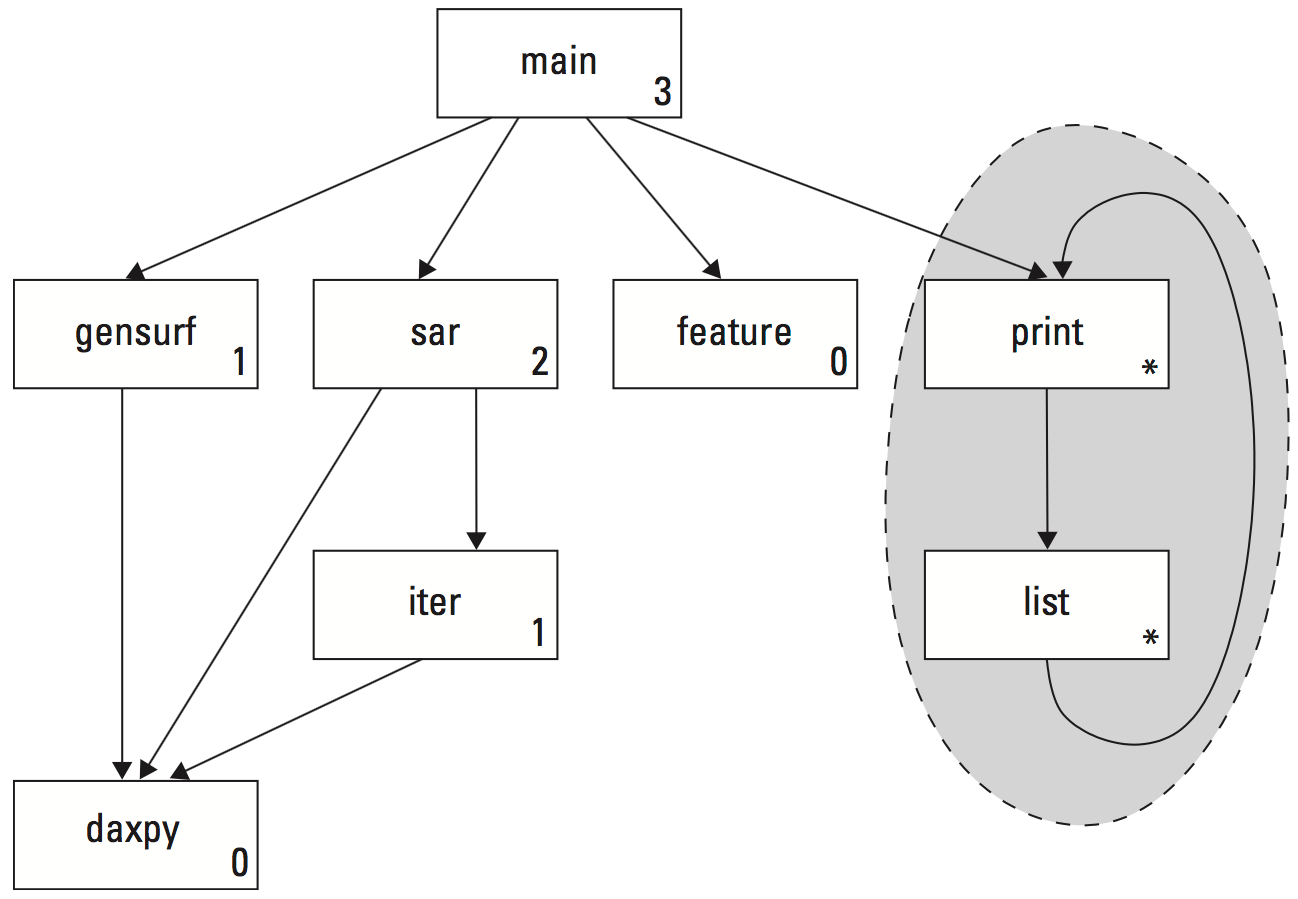
\includegraphics[width=0.6\textwidth]{img/f4-4.png}
				\caption{Análise de funções na qual os comandos \texttt{print} e \texttt{list} repetem inúmeras vezes.}
				\label{fig:perf_print_list}
			\end{figure}

			O exemplo da Figura \ref{fig:perf_print_list} mostra que as funções \texttt{print} e \texttt{list} formam um componente fortemente conectado e são marcados com um *. Em seguida, os vértices restantes de $ G $ são assinalados por uma regra ordinal,

			$$
			\text{ord}(u) =
			\left\{\begin{matrix}
			0 & \text{se nó } u \text{ é uma folha} \\
			\underset{(u,v) \in E(G)}{\max}\ \{ \text{ord}(v) \} + 1 & \text{caso contrário}
			\end{matrix}\right.
			$$


	\subsubsection{Modelo \textit{Multithread}}
		Além do modelo coprocessado, tem-se o modelo \textit{multithreads} que emerge como uma importante técnica de programação utilizada até em computadores com multiprocessadores. Neste modelo, o paralelismo natural do \hardware\ é conhecido e o \designer\ reconhece que o processador e os componentes executam continuamente. A coordenação desses componentes é manuseada por comunicações primitivas que tem sido desenvolvidas por processo concorrentes como semáforos, mensagens e outros. Cada \hardware\ é considerado um componente que executa como uma \textit{thread} paralela e o sistema de semáforos é utilizado para deixar o sistema consistente e assim, ao invés de bloqueado, o \hardware\ conceitualmente fica em bloqueio esperado pelo semáforo ou por uma mensagem.


	\subsubsection{Modelo de Rede em Chip}
		Este modelo investiga o estado distribuído completamente e depende da troca de mensagem para explicitar o estado. A coordenação é implícita com a transferência de estado. Como é assumido que o \design\ referencial de \software\ foi construído com comandos de troca de mensagem explícita, não se considera em um manual de sistemas embarcados. Entretanto, tem-se visto que técnicas de alta-performance continuam filtrando-se para o nível de sistemas embutidos.


\section{Programação Linear Inteira (PLI)} \label{sec:pli}
	Este problema representa um subgrupo da programação linear no qual algumas ou todas as variáveis do problema pertencem ao conjunto dos números inteiros. A tentativa de solucionar um PLI para um modelo puro com quantidades de restrições é um problema $\mathcal{NP}$-difícil.

	Um modelo de PLI pode ser obtido com a seguinte característica:

	\begin{equation}
			\begin{array}{rrcll}
			\text{min}  &  c' x    &  ~     &  ~            &  ~               \\
			subject\ to &  a'_i x  &  \leq  &  b_i,         &  \quad i \in M_1 \\
			~           &  a'_i x  &  \geq  &  b_i,         &  \quad i \in M_2 \\
			~           &  a'_i x  &   =    &  b_i,         &  \quad i \in M_3 \\
			~           &  x_j     &  \in   &  \mathbb{Z},  &  \quad j \in N_1 \\
			~           &  x_j     &  \in   &  \mathbb{Z},  &  \quad j \in N_1 \\
			\end{array}
            \label{eq:constraints_pli}
	\end{equation}
    
    onde:
    
    \begin{description}
    	\item [$c'x:$] é uma função linear de custo;
    	\item [$x:$] variáveis de decisão;
    	\item [$a':$] coeficientes fixos;
    	\item [$a'x \leq b, a'x = b$ e $a'x \geq b:$] restrições para validação da solução.
    \end{description}


\section{Questões} 

	\subsection{\textit{Profiling}} \label{sec:dificuldades}

			Uma suposição não adequada com a formulação analítica é que ela usa informação de \textit{profile} para aproximar o tempo de fração que uma aplicação gasta em uma sub-rotina ou bloco básico, mas no entanto, várias situações podem gerar resultados enganosos.



		\subsubsection{Execução Dependente de Dados}

			Quanto um simples conjunto de dados não representa o tempo gasto de cada sub-rotina quando este é alterado a sub-rotina não terá mudanças substanciais com a mudança do dado de entrada. A detecção da situação onde um único conjunto de dados não é representativo torna a situação difícil e requer que o \designer\ do sistema compreenda a operação fundamental da aplicação como é o caso da análise de complexidade das rotinas. É possível analisar esses casos com alguns métodos sendo a análise manual dos algoritmos e suas operações básicas, a coleta de informações \textit{profiling} baseado em diferentes conjuntos de dados ou mesmo a tentativa de separar a aplicação talvez ao longo dos limites do módulo e fazer o \textit{profile} de cada módulo independente.

		\subsubsection{Comportamento Correlacionado}

			Outra questão surge em aplicações que explicita o uso de eventos cronometrados. Muitos \textit{profile} assumem que a aplicação fará um progresso estável em direção à solução mas algumas aplicações incorporam o tempo. Sistemas de \textit{profiles} usam um temporizador de intervalo para amostrar o contador de programas dependendo da aplicação para não serem correlacionados estatisticamente com o temporizador. No entanto, se a aplicação possui operações executando em tempos regulares, periódicos, então os resultados do \textit{profiling} podem ser considerado enganosos. Por exemplo, se uma aplicação é executada a cada 10ms e a amostragem é feita a cada 10ms, então o \textit{profiler} não fornecerá dados concretos referentes ao sistema.



		\subsubsection{Comportamento Faseado}

			Sobre a totalidade de sua execução, o controle se move entre \textit{clusters} de operações relacionadas, isso é, a execução de uma aplicação exibida localmente. Como um exemplo, consideremos uma aplicação que possui três rotinas. Assumindo que cada possui $ 33\% $ de tempo de execução, e que cada tem a possibilidade de ter um \speedup\ de 50\% e postas de forma ordenada da primeira à última. Se existe espaço somente para uma rotina em recursos de FPGA, então o \speedup\ máximo será de 12\%. Mas se o comportamento faseado é suportado pelo \design\ de sistema, então há mais opções. Um é olhar procurar itens em comum sobre os três \textit{cores} e uma segunda é um \hardware\ multiplexado por tempo. Não há abordagens automáticas para esse.



		\subsubsection{Efeitos de I/O}

			\textit{Profiles} não contam tempo de I/O tais como acesso ao espaço de usuário e dispositivos realizando algum procedimento de busca ou ação.



		\subsubsection{Números de Chamada}

			\textit{Profiles} entretanto continuará a calcular quando sub-rotinas são invocadas. É importante ter noção o quanto uma sub-rotina é invocada.

	\subsection{Estrutura de Dados}

		Design de referência de \software\ naturalmente reflete um viés em relação às implementações em \software. Isso é compreensível, já que a programação é ensinada no contexto de modelo de computação sequencial ordinário. Com esses modelos, a diferença entre

	\begin{verbatim}
	while( i!=NULL ) {
	  proc(i) ;
	  i = i->next ;
	}
	\end{verbatim}
	e
	\begin{verbatim}
	while( i<n ) {
	 proc(x[i]) ;
	 i=i+1;
	}
	\end{verbatim}

		é insignificante já que ambos tomam $ \mathcal{O}(n) $ passos, mas em nível de \hardware\ o último pode ser mais desejável sendo no mínimo, uma ampla janela de pré-busca é possível. Se pudermos determinar que, em várias iterações do ciclo, cada \texttt{proc(x[i])} é independente, então pode-se melhorar o \design\ por meio de \textit{pipeline} ou paralelismo regular.

		O \design\ de referência de \software\ serve como extremamente bem como uma especificação, mas se executar um \textit{profile} do \design\ de referência, não será capturado os benefícios da implementação pois esses benefícios provem de alterações algorítmicas e são improváveis de serem reveladas por técnicas automáticas. Consequentemente, cai sobre o \designer\ de sistema compreender ambos o algoritmo de \software\ implementado no \design\ referencial e como pode ser re-implementado em \hardware.

		Há vários formas comuns de estruturas de \software\ que pode ser rearranjadas para produzir melhor \design\ de \hardware. Estruturas de dados que utilizam ponteiro como listas encadeadas, árvores, etc. podem ser representadas por uma estrutura ``\textit{flat}'' como vetores e arranjos produzindo acesso regular em memória que podem ser pré-buscadas subsequentemente ou utilizadas em \textit{pipeline}. Outra forma de ganho de performance é no tamanho de bit. Programadores de \software\ geralmente assumem um valor fixo, mesmo que utilizem somente poucos bits de informação. Enquanto \software\ tem caminho de dados fixos e relativamente baixa largura de banda entre componentes, \hardware\ se destaca no gerenciamento de largura de bits arbitrárias sendo possível alavancar grande largura de banda fornecida pela interconexão programável do FPGA.

	\subsection{Manipulando Tamanho de Recurso}

		A mudança mais simples envolve quebrar uma sub-rotina em sub-rotinas menores fazendo com que o recurso em \hardware\ fique menor e mais fácil de ser implementado.

		Há três momentos que agregar sub-rotinas são necessárias. Se duas sub-rotinas tomam 25\% cada uma do tempo da aplicação, então elas são candidatos fortes para a implementação em \hardware. No entanto, se for implementado individualmente, cada uma invoca o custo da sua interfaceação. Se há três sub-rotinas relacionadas (uma invocando a próxima), então a combinação delas pode reduzir o custo de invocações. Entretanto, o custo da interface não é sempre insignificante e vale a pena o esforço do usuário para investigar a situação.

		Qualquer outra mudança é substancial. Frequentemente, implementação em \hardware\ tem performance significativa por ter formato de dados de dados específicos da aplicação. Para que o \software\ seja mais eficiente nos formato de dados não padronizados, programadores irão investir em estruturas de dados que não são bem mapeadas para o \hardware. Assim, vale a pena olhar para o propósito e considerar a substituição de estruturas de dados para melhor explorar o \hardware.





\begin{comment} %comment Módulos e Interfaces em \Design\ de \Software
\section{Conceitos e Componentes de \Design\ de Sistemas}
% \subsection{Módulos e Interfaces}
%Existem duas filosofias de \design\ para a construção de um sistema. Em um delas é possível realizar a especificação de cada função do projeto, chamado de blocos básicos\footnote{Um bloco básico é uma sequência maximal de instruções sequenciais com \textit{single entry and single exit} (SESE).}, e conectá-los logicamente de acordo a fim gerar o sistema completo. Tal é descrito como abordagem \textit{bottom-up}.
%A segunda baseia-se na descrição de um sistema completo e geral sendo que, em seguida, o \designer\ desmembra-o definindo seus sub-blocos até chegar ao nível mais básico de suas funções. Essa é chamada de abordagem \textit{top-down}.
%O conceito de abordagem de desenvolvimento de projetos é importante para descrever os conceitos de módulo e interface.%, segundo \citet{Sass2010}.

\subsection{Módulos e Interfaces em \Design\ de \Software}
\citet{Sass2010}, em seu livro, descreve que módulo é qualquer conjunto de operação auto-contidas que possui um nome, interface formal e geral e alguma descrição funcional. Isso significa que qualquer procedimento, mesmo que em \software\ ou em descrição de \hardware, que possa ser representado por uma caixa graficamente é considerado um módulo.
Define-se por interface formal o nome do módulo e a enumeração de duas operações, incluindo suas entradas e saídas, caso existam e a interface geral inclui todas as características da interface formal e qualquer protocolo ou comunicação adicional implícita. Com a interface formal descrita, é possível realizar inspeções mecânica e técnica no módulo enquanto a geral, o entendimento desse em alto nível.
Por último, um módulo pode ter também uma descrição funcional no qual pode ser implícita, formal ou informal. Quando a descrição é implícita, a descrição está presente de forma clara no nome do módulo, como por exemplo \texttt{full\_adder}. A formal consiste na documentação ou em meios matemáticos e comentários formais sobre as operações do módulo e a informal pode ser comentários descritivos ao longo da escrita da função.

Outros termos importantes são implementação e instância. Uma implementação é a realização de uma funcionalidade pretendida de um módulo mesmo que este tenha várias implementações como é permitido num ambiente de descrição de \hardware\ criar várias arquiteturas diferentes para um mesmo módulo.
Já a instância é o uso de uma implementação.
Enquanto em instâncias em nível de \software\ imagina-se relações um-a-um entre implementação e instância, em \hardware\ é comum o uso de copias físicas de cada implementação, sendo cada cópia representa uma instância no final. Na Figura \ref{fig:instance} é possível ver em \textit{a)} um instância padrão de uma implementação e em \textit{b)} uma outra instância com uma identificação única.

\begin{figure}[h] \centering
\includegraphics[width=0.7\textwidth]{img/f3-2.png}
\caption{Instâncias e suas descrições. Fonte: \cite{Sass2010}.}
\label{fig:instance}
\end{figure}

Como exemplificação, pode-se construir um somador completo de 4-bit utilizando várias instâncias da implementação do somador completo de 1-bit, exibido na Figura \ref{fig:somador_instancias}.

\begin{figure}[h] \centering
\includegraphics[width=0.98\textwidth]{img/f3-3.png}
\caption{Somador completo 4-bit utilizando instâncias de 1-bit. Fonte: \cite{Sass2010}.}
\label{fig:somador_instancias}
\end{figure}
\end{comment}

\begin{comment}
\subsection{Abstração e Estado}
\subsection{Coesão e Acoplamento}
\end{comment}




\begin{comment}
\section{Publicações}

	Neste apêndice são listados os trabalhos publicados em eventos científicos desenvolvidos durante o período de realização da presente pesquisa.

	\begin{enumerate}
		\item a
	\end{enumerate}

	O trabalho a seguir foi submetido e aceito para publicação em eventos científico.

	\begin{enumerate}
		\item  a
	\end{enumerate}
\end{comment}

\begin{comment}
\section{Reprodutibilidade}

	O código fonte do resolvedor desenvolvido no presente trabalho foi disponibilizado no seguinte endereço \todo{url.rar}. Convido o leitor interessado a validar os resultados obtidos bem como dar continuidade ao trabalho. A Tabela \ref{tab:parametros} apresenta uma lista de parâmetros que podem ser passados ao resolvedor via linha de comando.

	\begin{table}[H]
	\caption{Lista de parâmetros para o resolvedor}
	\begin{tabular*}{20cm}{lp{12cm}}
	-xml= & Arquivo de entrada para o resolvedor (obrigatório) \\
	-out= & Arquivo para o qual a solução obtida será salva (obrigatório) \\
	-time\_limit= & Limite de tempo de execução em segundos (obrigatório) \\
	-seed= & ``Semente'' aleatória (obrigatório) \\
	-alg= & Seleciona o algoritmo a ser aplicado (obrigatório) \\
	\\
	-bl\_max & Máximo de iterações do método de descida (Não Ascendente Randômico) \\
	\\
	-sa\_max & Máximo de iterações por temperatura no algoritmo SA \\
	-sa\_alpha & Razão de esfriamento do algoritmo SA \\
	-sa\_tempini & Temperatura inicial do algoritmo SA \\
	-sa\_tempmin & Temperatura mínima do algoritmo SA (usualmente 0)\\
	-sa\_reheats & Número de reaquecimentos do algoritmo SA\\
	\\
	-ils\_max & Máximo de iterações por temperatura no algoritmo SA \\
	-sa\_alpha & Razão de esfriamento do algoritmo SA \\
	-sa\_tempini & Temperatura inicial do algoritmo SA \\
	-sa\_tempmin & Temperatura mínima do algoritmo SA (usualmente 0)\\
	-sa\_reheats & Número de reaquecimentos do algoritmo SA\\


	\label{tab:parametros}
	\end{tabular*}
	\end{table}

\end{comment}

\end{appendices}
\let\cleardoublepage\clearpage
%% Produce the un-numbered back matter (e.g. colophon,
%% bibliography, tables of figures etc., index...)
\begin{backmatter}
	%!TEX root = ../Dissertacao.tex

\bibliographystyle{kluwer}
\bibliography{bibliography}
\printindex
\end{backmatter}

%% Close
\end{document}
